%
% TU/e Style Master Thesis template for LaTeX
%
% 2021 Crated by Marko Boon to new corporate identity,
% Based on a template by Thijs Nugteren and Joos Buijs.
%
% THIS IS THE MAIN FILE (i.e. compile this file, compiling the others directly won't work)
%
\documentclass[a4paper,10pt,twoside]{book}				% Base document class
\usepackage{tuethesis2021}								% Modified TU/e Thesis format
\usepackage[utf8]{inputenc}								% Enables UTF-8 characters
\usepackage[english]{babel}								% "Culturally determined typographical rules"
\usepackage{datetime}									% To make the month automatic
\usepackage{booktabs}									% Nicer tables
\usepackage{multirow}                                   % Multirow in tables
\usepackage[backend=biber]{biblatex}					% Bibliography
\usepackage{subcaption}									% Subfigures. Why the package is called subcaption? 🤷🏻‍♂️
\usepackage{dsfont}										% \mathbb{1} doesn't work
\usepackage[linesnumbered,ruled,vlined]{algorithm2e}	% Algorithms
\usepackage{microtype}									% Nicer micro type adjustments, but disabled during draft due to much longer compile times

% ------------------------ Bibliography ------------------------
\addbibresource{references.bib}

% ------------------------ Automatic Datetime ------------------------
\newdateformat{monthyear}{\monthname[\THEMONTH] \THEYEAR}


% ------------------------ TITLE PAGE ------------------------
% These commands need to be defined in order to produce a correct and personalized document.

\newcommand{\doctitle}{Towards domain agnostic Wi-Fi CSI gesture classification}
\newcommand{\shortitle}{Domain Agnostic Wi-Fi CSI Gesture Classification}
\newcommand{\docsubtitle}{Master's Thesis}
\newcommand{\me}{Yvan Putra Satyawan}
\newcommand{\version}{}
\newcommand{\placeMonthYear}{Eindhoven, \monthyear\today}
\newcommand{\department}{Department of Mathematics and Computer Science}
\newcommand{\group}{Interconnected Resource-aware Intelligent Systems Research Group}
\newcommand{\firstCommitteeMember}{Prof. Dr. Ir. Nirvana Meratnia} % use all the titles for your committee members!
\newcommand{\secondCommitteeMember}{Bram R.D. van Berlo, M.Sc} % usually the daily supervisor
\newcommand{\thirdCommitteeMember}{} % usually the external member
% ------------------------ TITLE PAGE ------------------------

\begin{document}
% The title page will be inserted automatically, here.

\clearpage

%Sometimes line numbers are nice, uncomment the next line to enable:
%\linenumbers

\chapter*{Abstract}\label{chapter:abstract}

Somewhat ominously, we are getting closer and closer to ubiquitous remote sensing and gesture recognition through the use of only Wi-Fi signals.
This is understood as the ability to recognize gestures performed by an individual with nothing more than the interference their bodies provide to surrounding Wi-Fi signals.
The main challenge facing the mainstream adoption of such technologies is the lack of generalizability seen in published models against various domain factors.
This work aims to bring us closer to such a (dystopian) future where such technologies may be mainstream by presenting DARLInG, a novel approach to domain shift mitigation through the use of domain auto-labeling using reinforcement learning.
We show that this may be a promising approach for domain shift mitigation, although further research is necessary to investigate whether this approach will actually be applicable in mainstream applications.

\chapter*{Acknowledgements}\label{chapter:acknowledgements}

I would like to express my gratitude to the following:

To my supervisors Nirvana and Bram for giving up their time to guide me, and quite thoroughly, through this thesis,

To my friends, those of you in the DSAI masters with me and our group Belly Dancing as a Service and those of you in Pattern.

To my family, who supported me throughout the entirety of my masters.


\tableofcontents

\listoffigures

\listoftables

\mainmatter

\chapter{Introduction}\label{chapter:introduction}

\begin{figure}[b]
	\centering
	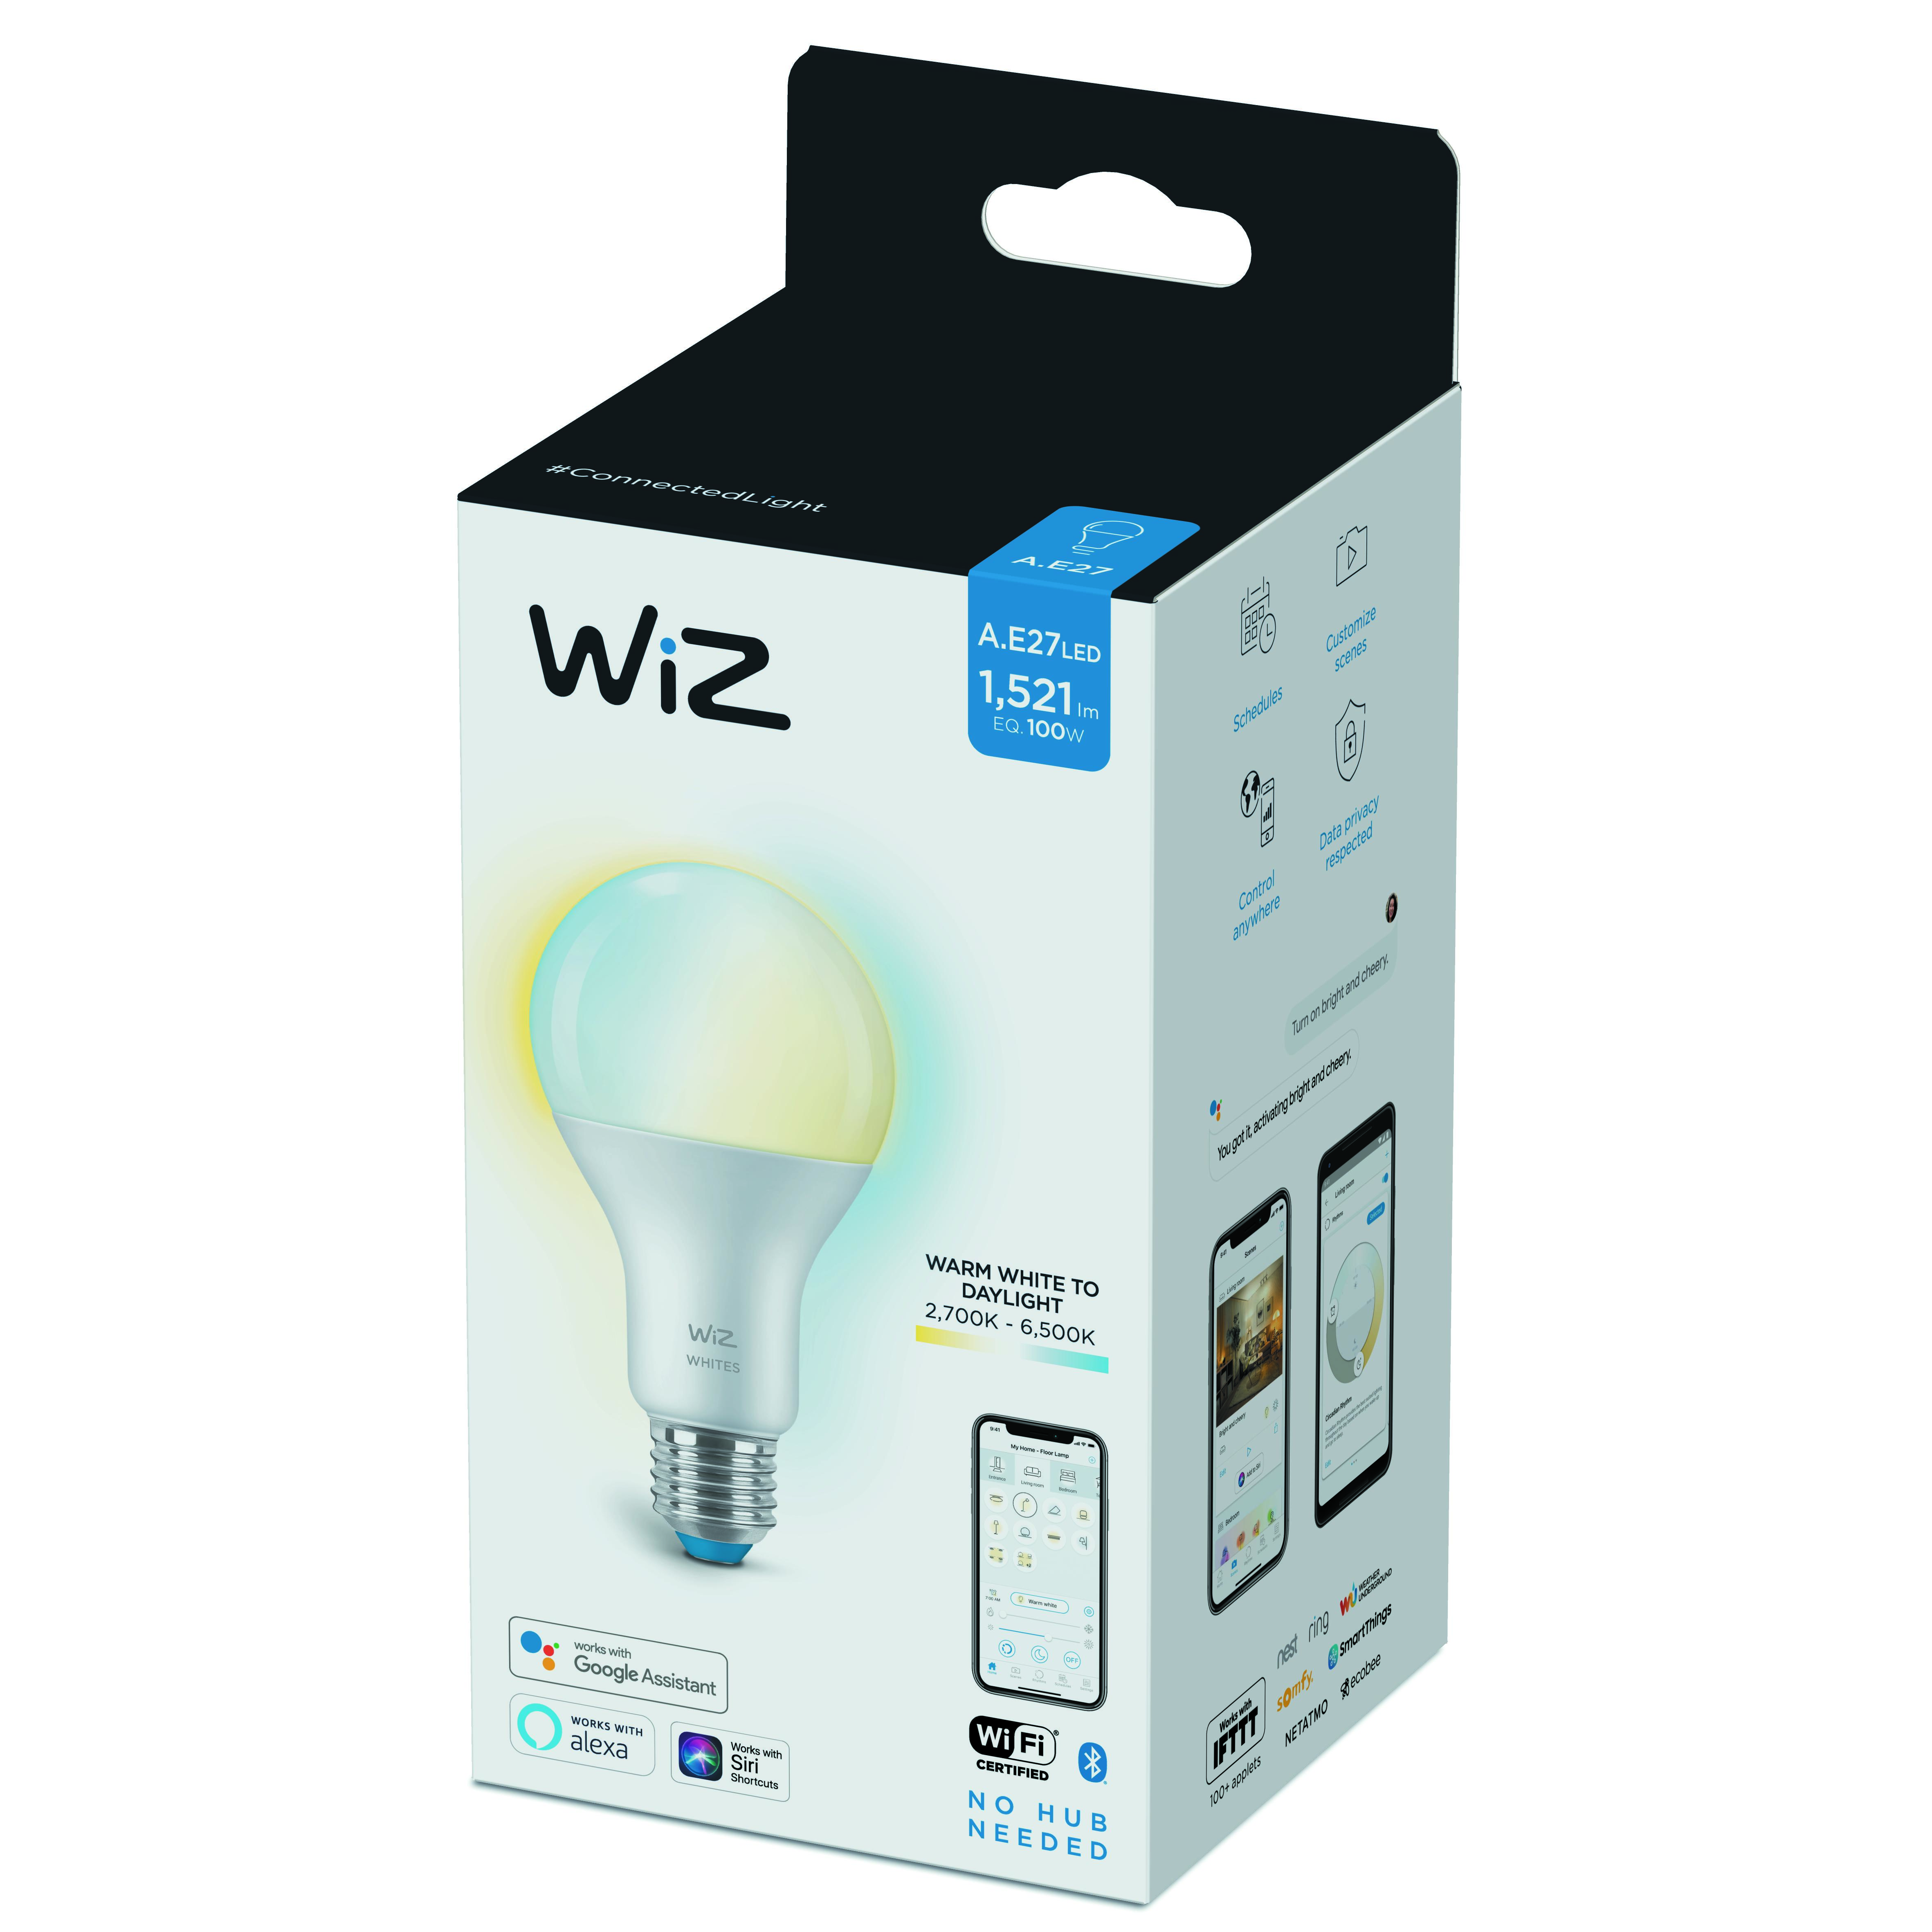
\includegraphics[width=0.3\linewidth]{figures/wiz-a60-tunable-white}
	\caption{A WiZ A60 Tunable White light bulb, one example of an IoT smart device with an integrated Wi-Fi Radio \cite{signify2020wiz}.}
	\label{fig:wiz-lightbulb}
\end{figure}

In this ever more connected climate that we find ourselves in, IoT devices everywhere are adding little conveniences to our every day lives.
With IoT devices becoming ever more common and reaching a forecasted 27 billion devices by 2025 \cite{hasan2022state}, the dream of ubiquitous computing and sensing is transitioning from a mere dream to the reality of our every day lives.
Additionally, approximately 19\% of new devices bought in 2020 also utilize some form of Wi-Fi radio for communications with a forecasted increase to 24\% by 2025.

It is clear that this trend towards integrating computing technology into everyday objects will only accelerate in the future.
The increased convenience and efficiency may be the biggest boon of such technologies.
For example, smart thermostats can predict heating requirements and adjust accordingly, leading to lower heating costs in a house while maintaining the convenience of having a well heated space.

With all these connected devices becoming and edge computing ability comes ubiquitous sensing, enabling new modalities of interaction and improving data collection and analytics.
It is now possible to envision households with complete presence detection coverage, for example, through the use of smart motion sensors, enabling increased efficiency by intelligently identifying which rooms require heating and lighting and which do not.
Always-on voice control systems, such as Amazon Alexa and Google Assistant speakers are also increasingly common, making a connected AI-assistant only one call away.
The always-connected nature of these sensors also enable the gathering and analysis of vast amounts of user data, potentially providing valuable insights into various aspects of our lives.

One challenge that has continued to plague ubiquitous devices is the lack of a ubiquitous user interface which does not require input devices.
It is not too common to use the end device itself as the input.
Even in the case of voice control systems, a dedicated smart speaker is still required and must be placed in every room from which interaction is desired.
For example, in the case of smart lights or smart thermostats, the end device would be the light bulbs and heating system, respectively.
In both cases, a separate control unit, the light switch or thermostat, respectively, is still required.

With these challenges in mind, Wi-Fi-based sensing provides one potential solution.
Many IoT devices already contain some sort of Wi-Fi radio, such as the Phillips Hue Light bulb in Figure \ref{fig:wiz-lightbulb}, and it would be a rather safe assumption to make that spaces with IoT devices would also have some sort of Wi-Fi infrastructure in place as well.
With this in mind, the idea of a gesture-based interface based around Wi-Fi becomes rather appealing.
The use of Channel-State Information (CSI) also enables of finer-grain signals to be extracted from consumer-grade Wi-Fi radios, enough to enable reliable gesture recognition \cite{adib2013see}.
This method does, though, suffer from the domain-shift problem, achieving the best accuracy only in cases with a prediction model fine-tuned to a specific person and environment is used.

With this thesis, we aim to explore the use of CNN architectures and domain-shift mitigation methods to improve the state-of-the-art in Wi-Fi CSI-based gesture classification.
Specifically, we will look at using preprocessing methods to transform the input signal from CSI into an image using table-to-image and signal-to-image transformations, the use of traditional signal processing algorithms to process the incoming CSI signal, and the use of Reinforcement Learning (RL) to perform domain auto-labeling and provide the CNN classifier with additional information.

\section{Context and Background}\label{sec:intro-context}

IoT devices are without a doubt increasingly prevalent in everyday life.
The Atlas building at the Technical University of Eindhoven (TU/e), for example, uses centrally networked lights for all of its lighting fixtures powered through Power over Ethernet (PoE) and this is at least partially credited as a reason the building has the best efficiency of any academic building in Europe when it was constructed \cite{tue2019atlas}.

All over the building, presence detection, in the form of motion detection sensors, is also used to automatically set appropriate lighting levels for each room.
This is just one example of how ubiquitous computing and sensing has now entered the mainstream and is no longer a dream of a few enthusiasts and IoT evangelists.
Developments in AI and big data processing has also made the usefulness of ubiquitous computing much more evident, legitimizing its use in everyday objects.

Finally, the deployment of 5G networks in densely populated areas is working towards enabling faster speeds and lower latency, essential in many ubiquitous computing and sensing applications.

With these advances, the question has shifted towards what sort of interface we should utilize to provide an always-available non-intrusive experience for the users.
One possible solution is gesture-based interfaces.
With any ubiquitous computing and sensing product, especially in the consumer space, minimal setup on the user's part is desired; otherwise the product will not become something which is widely accepted and used.

Wi-Fi gesture recognition can solve these issues, providing a gesture-based interface requiring potentially zero additional setup requirements.
As a bonus, this would also be a low-cost solution which many IoT devices already having the necessary hardware for regardless.

There also exists a task group for Wireless Local Area Network (WLAN) sensing, called 802.11bf, within the IEEE 802.11 working group, the group which sets the standards for WLAN, with members from large companies including Huawei, Qualcomm, and Meta \cite{du2022overview}.
This shows there is genuine interest in the industry to utilize WLAN for these purposes.
With an approval date set for September 2024, it is clear that WLAN sensing is not just some theoretical possibility confined to a lab, but rather a very real technology that may soon become widespread.

To make such an approach possible, we utilize machine learning (ML) to process the incoming CSI data and classify user gestures.
Wi-Fi technology, while being very different to radar technology, are both forms of radio technology.
Although topologically very different, it naturally, or not so naturally, follows then, can Wi-Fi be used for remote sensing?
The answer to this question, according to \cite{adib2013see} and \cite{chetty2011through}, the answer is a resounding yes!

There are even commercial products which have become available on the commercial market during the writing of this very thesis that incorporates parts of this technology. 
Signify's line of WiZ smart lights uses \textit{SpaceSense} technology, which is a proprietary algorithm that detects motion through ``disturbances [in the Wi-Fi signal] created by a person's presence'' and is available through a software update \cite{signify2023spacesense}.
It should be noted, though, that this is only capable of presence detection and not of gesture recognition.

However, ML suffers from degraded performance when faced with domain-shifts.
When dealing with new, unseen users and environments, gesture classification accuracy degrades significantly \cite{chetty2011through,adib2013see,pu2013whole,adib20143d,he2015wig,jiang2018towards,zheng2019zero,jiang2020wigan,ma2021location}.
As such, factors to mitigate this domain-shift problem are required in any implementation outside of a pristine laboratory setting.

For the purposes of our thesis, the Wi-Fi information we utilize for gesture classification is known as the Channel State Information (CSI).
This comes in the form of a set of complex numbers denoting signal differences for each receiver access point (AP) from each transmitting AP.
This complex number can then be represented as a set of amplitudes, or radii, and phase shifts, or angles, when considered as polar coordinates on the complex plane.
CSI itself is a description of the multipath effects of a signal traveling from the transmitting AP to the receiving AP.
In the realm of WLAN, the estimated CSI of incoming signals is used to correct for these multipath effects, making it possible for the system to adapt to current environmental conditions.
Importantly, human activity in an environment also affects the CSI, making it possible to infer activity through CSI.

\section{Motivation}\label{sec:intro-motivation}

There are significant potential commercial and practical benefits to enabling domain-agnostic Wi-Fi gesture classification.

The upcoming release of the 802.11bf standard, which standardizes the requisite hardware technology for Wi-Fi sensing, marks a pivotal moment from a commercial standpoint. To fully exploit these emerging technologies, it is of utmost importance to investigate their practical applications.

Wi-Fi sensing is also unique in that the hardware for it is already commercially available and widespread, though not necessarily standardized.
As such, it is in a unique place where it is an almost completely software-based solution for preexisting, mass-adopted hardware enabling completely new modes of interaction.
This makes it unique and, ultimately, much more commercially desirable as a technology to be adopted.

With respect to domain-agnosticism, the motivating factor is that the largest hurdle for Wi-Fi gesture classification is its loss of performance in new, unseen domains.
A model that cannot adapt to such issues will inevitably be nonviable for commercial adaptation lest the end-user be required to perform the same gesture hundreds of times in various positions after installing every single smart IoT device.

We also wish to further the state-of-the-art in domain-agnostic models.
The results of this thesis is not only applicable to the field of Wi-Fi gesture classification.
Domain-agnostic systems are required for many industry applications, such as for patient sensing in healthcare, for consumer behavior tracking in retail, and for hands-free control of smart IoT devices in consumer homes.
The conclusions of this thesis will hopefully be able to advance the field and provide new insight into what future avenues of research may end up being fruitful.

Finally, a Sci-Fi future where all your devices are controlled through your thoughts might seem like a dream, but in reality, we are not too far from this future.
The use of Wi-Fi sensing to detect gestures is one step closer to this futuristic dream and in addition to all the potential commercial and practical benefits this technology could bring, the sheer ``coolness'' of the technology should not be underestimated as a motivation to perform research.

\section{Problem Statement}\label{sec:intro-problem-statement}
Models already exist to classify gestures through Wi-Fi CSI data.
Ideally models are solely influenced by those factors which contribute to the correct classification of the gesture, this is, in reality, not the case.
These models are susceptible to the influence of ``domain factors'', encompassing variables such as the identity of the gesturing subject and the surrounding environment in which the gesture is performed.

These domain factors cause feature domain shifts between the training data and the data encountered during actual use or inference despite both domains containing the phenomenon of interest, for example the gesture we wish to classify.
Due to these shifts, performance of the model is degraded \cite{chetty2011through,adib2013see,pu2013whole,adib20143d,he2015wig,jiang2018towards,zheng2019zero,jiang2020wigan,ma2021location}.
It is thus interesting to be able to create a domain-agnostic model whose output is independent of the aforementioned domain factors.

There exist proposals to mitigate this degradation including using very large datasets.
This is one method especially championed by large companies such as Tesla and OpenAI which have vast resources at their disposal.
However, the gathering of such large datasets is only feasible for specific scenarios.
In the case of Tesla, for example, having a large fleet of vehicles capable of recording what is essentially supervised training data makes it possible to collect the vast amounts of data required to build a dataset usable for the training of self-driving vehicles \cite{tesla2017data}.
Various OpenAI projects, on the other hand, simply scrape large amounts of websites and collect these as part of their dataset \cite{brown2020language}.
Within the scope of our research, due to its nature, such widespread data collection methods are non-viable, and we must resort to more novel approaches towards data-agnosticism.

Most alternative methods to simply using very large datasets rely on a ground truth domain label being provided \cite{jiang2018towards,xue2020deepmv}.
In these approaches, a ``discriminator'' network is used to predict domain labels from the latent embedding of the data and an adversarial training procedure is then used.
The ``generator'' which produces these latent embeddings must thus generate embeddings which contain no domain information while still maintaining enough information that a classifier model can use its output to correctly classify target features.

In \cite{ma2021location}, a method is presented which does not require manually labeled domain labels to be provided.
Instead, a CNN encoder and state machine neural network are used and their output is fed into a recurrent neural network (RNN) to provide a classification.
The RNN is trained through reinforcement learning (RL) to predict features correctly and independently of domain factors.

We hypothesize that we can extend the RL component of \cite{ma2021location} to facilitate domain auto-labeling and eliminate the use of a state machine neural network by using signal-to-image preprocessing methods.
Towards these goals, we specify our research questions as follows:

\begin{enumerate}
	\item To what extent can a reinforcement learning agent utilize the latent signal representation produced by the CNN to accurately produce a latent representation of the domain space, measured by performance metric difference in a domain factor leave-out cross validation setting between a classifier provided the domain space representation and one which has not?
	\item To what extent would changing the latent representation of the domain space from a one-hot encoding to a probability measure affect the performance of the classifier, measured by the performance metric difference in a domain factor leave-out cross validation between both domain space representation types?
	\item To what extent can signal-to-image transformation replace the state machine neural network presented in \cite{ma2021location}, measured by comparing the performance metric difference in a domain factor leave-out cross validation setting between the model presented in \cite{ma2021location} and our approach provided no self-label?
\end{enumerate}

The rest of this thesis will present a literature review, background on required knowledge, the proposed methodology, experimental results, and discussions and conclusions of those results.
\chapter{Literature Review}\label{chapter:literature-review}

In this chapter we review important works in the literature which form the foundation of this thesis.
We first discuss the initial set of works which cover Wi-Fi activity detection as well as other related works which do not use CSI data specificially before discussing those works which do utilize CSI data and publicly available datasets for this purpose.
We then look at various signal-to-image transformation methods which may be applied to time-series signal data, enabling the use of techniques from the image processing domain.
Finally, we look into domain shift mitigation methods and specifically reinforcement learning for domain shift mitigation.

\section{Wi-Fi for Activity Detection}

Past works have investigated the use of Wi-Fi signals generally for the purposes of activity detection.

The first work regarding the use of Wi-Fi signals for the detection of humans subjects we could find is the work of Chetty, Smith, and Woodbridge in 2012 \cite{chetty2011through}.
Their work utilized passive Wi-Fi signals propagating through a building with receivers placed outside the building for presence detection.
This method achieved reasonable results and proved that Wi-Fi signals could be used to detect human presence in buildings, although it required the indoor and outdoor APs to be synchronized through wires and was unable to detect precise activities of the human subjects.

The first work we could find discussing the use of Wi-Fi for activity detection is the work from Fadel Adib and Dina Katabi, published in 2013 \cite{adib2013see}.
This work shows the potential of using signals which could be produced by Wi-Fi APs to detect human activity from through a wall.
The most important idea in this work is the elimination of the radio ``flash'' which comes with the signal hitting a wall and bouncing back towards the transceiver.
Their work focused more on the radar technology implications and not on the use of consumer Wi-Fi APs for gesture detection.
They did, though, show that using matched filters was enough to perform rudimentary gesture recognition, given coarse enough gestures.

In the same year, a different group published a paper showing how to use signals in the 2.4 GHz range, i.e., compatible with Wi-Fi transceivers, for simple gesture detection using Doppler shift identification \cite{pu2013whole}.
This paper proposes the use of a narrowband pulse with a very narrow bandwidth of only a few Hertz and detecting the Doppler shift from the returned signal.
Using this method, the researchers were able to identify 9 different gestures with a claimed 94\% accuracy.

The same group as \cite{adib2013see} also published a separate paper in 2014 detailing the use of a custom-built Wi-Fi based device which could detect course body motions by leveraging the geometric position of its antennas and measuring values through a Time of Flight (ToF) approach \cite{adib20143d}.

Finally, it is also important to note that IEEE has a task group 802.11bf assigned specifically to standardize Wi-Fi sensing technologies \cite{du2022overview}.
This group is focused on standardizing the hardware requirements, specifically enabling CSI accessibility and specific measurement procedures which future devices can implement.
Their target is to standardize these requirements for future devices both in the sub-7 GHz range and in the 60 GHz range.
They additionally provide suggestions for what methods can be then be used to interpret the data provided, including the use of Fast Fourier Transform (FFT) algorithms to calculate a Channel Impulse Response from CSI and a Doppler FFT, which may be directly used for gesture recognition.
The standards for 802.11bf is set to be ratified and published by September 2024.

\section{Wi-Fi CSI for Gesture Recognition}

A selection of works which utilize Wi-Fi CSI data specifically for the task of gesture recognition are discussed in this section.

To the best of our knowledge, the first work discussing the use of CSI for gesture recognition was published in 2015 by He et al. \cite{he2015wig}.
This work looks into the use of CSI and outlier detection to detect gestures, achieving 92\% gesture recognition accuracy on four gestures in a line-of-sight experiment and 88\% accuracy in a non-line-of-sight experiment.

The 2019 work titled Person-in-WiFi from Wang et al. proposes the use of an array of three transmitter and three receiver antennas to directly predict body segmentation and pose estimation of persons located in between the aforementioned antennas \cite{wang2019person}.
In this work, they used an RGB camera to provide ground truth annotations.
The ground truth body segmentation masks were generated using Mask-RCNN while the Body-25 model of OpenPose was used for pose detection.
This work, shows that body segmentation and pose estimation is possible with only CSI data, achieving an mAP of 0.38 for body segmentation and around 0.1 meter error for join estimation. 
Qualitatively, the results are quite impressive and it is clear that at the very least, the model performs well given that its input data is one-dimensional.

Using the same dataset, Geng, Huang, and De La Torre published DensePose in 2022 performs similarly, but instead produces UV coordinates of the subjects.
This work also provides some interesting preprocessing steps on the raw CSI data to improve prediction performance.

WiGAN, published in 2020, proposes the use of a Generative Adversarial Network (GAN) to augment training data using the generator as well as using the discriminator as a feature fusion and extraction module \cite{jiang2020wigan}.
The output of the discriminator is then used fed into a Support Vector Machine (SVM) which classifies then gesture seen in the input data.
The authors claim that by using the discriminator, which fuses together multiple layers of a CNN module through yet another convolution, their method is able to ``learn and recognize the importance of different depth features by itself''.
On publicly available datasets, WiGAN indeed achieves better results than the competing methods at the time, achieving 98\% accuracy on Widar 3.0 with known subjects and $\approx$8--10\% lower performance on new domains.

The same group, in the same year, published DeepMV which proposes the use of multiple APs and audio sources, in the form of ultrasound signals, with a domain discriminator and embedding generator \cite{xue2020deepmv}.
This work is based on the intuition that the fusion of sensor data from multiple APs and audio sources placed around the room, which intuitively should provide more data.
The embedding generator produces a latent representation of the action which can then be used by a fully connected module to classify the action being performed while the domain discriminator uses the latent representation to predict the domain of the action.
A minimax game is played between the embedding generator and domain discriminator to minimize the maximum accuracy of the domain discriminator while maximizing the minimum accuracy of the action classifier.
On their self-collected dataset, they were able to achieve 83.7\% mean accuracy, outperforming all other benchmarked methods.

The 2021 paper by Zhuravchak et al. proposes the use of an LSTM as a classifier \cite{zhuravchak2022human}. 
In this method approach, CSI data is provided as an input with a fixed length and the LSTM provides a single output representing the action detected within the input window.
Their method achieves 87.8\% accuracy on a self-collected dataset.

Ma et al., published in 2021, proposes the use of a CNN and neural network state machine encoder and a LSTM trained using RL to eliminate the need of domain specific information \cite{ma2021location}.
This work also contains a curated benchmark of many previous works in this field.
Their proposal is the use of a neural network state machine relies on the assumption that there is a temporal dependency within and across CSI segments.
For example, it is unlikely that a person who is currently standing will immediately be sitting within the next CSI segment without a sit-down transition segment in between.
Although unlikely, the probability is non-zero, due to incontinuities in the data and mislabeling in the ground-truth labels, and thus a neural network state machine is used.
The results show >97\% mean accuracy on in-domain test samples with a drop of 14--17\% on out-of-domain samples.

Additionally, a few bachelors thesis' fromt he past years at the IRIS research cluster at TU/e have focused on this problem as well.
The 2022 thesis by van den Biggelaar proposes the use of reinforcement learning with Deep Q-Networks as the gesture classifier \cite{biggelaar2022gesture}.
Their result shows $\sim$88\% mean accuracy on Widar 3.0, dropping by $\sim$4\% on out-of-domain test samples.

The 2022 thesis by Oerlemans compares how different preprocessing methods appear to affect gesture recognition performance \cite{oerlemans2022effect}.
Specifically, signal filtering through a finite impulse response filter and phase unwrapping, transformation to a Doppler frequency spectrum (DFS), and transformation using Gramian Angular Fields (GAF) was explored.
On the SignFi dataset, they show that each of the above steps do indeed significantly improve model performance with the GAF transformation coupled with signal filtering resulting in the best performance.

\section{Wi-Fi CSI datasets for Gesture Recognition}

Three Wi-Fi CSI datasets for gesture recognition were considered for this thesis and they are each explained in this section.

The Widar 3.0 dataset, forthwith referred to as the Widar dataset for brevity, presents a dataset with developed specifically for ``cross-domain learning solutions'' \cite{zheng2019zero}.
The solution provided in this dataset is two-fold: 1) the (relatively) high number of domains that the data was collected with, and 2) the proposal of Body-coordinate Velocity Profile (BVP) with is a theoretically domain-independent representation of the data.
More details of BVP is discussed in Section \todo{Desecribe in background section}.
Finally, this paper also provides a baseline model to compare against.

SignFi is a dataset of Wi-Fi CSI data specifically for sign language recognition \cite{ma2018signfi}.
This dataset contains over 276 sign gestures in a lab and home environment with five different users.
A baseline CNN model is also presented in this paper, capable of achieving a $\sim$87\% mean accuracy over 150 sign gestures.

Person-in-WiFi is the dataset used in the paper by Wang et al. \cite{wang2019person}.
This dataset was made public and includes both Wi-Fi CSI data and RGB camera data of the activity from a fixed position.
This dataset was collected specifically for pose estimation solutions and is not meant specifically for activity recognition, as no activity labels are provided in the dataset.

\section{Signal-to-Image Transformations}

Different preprocessing methods have been investigated to transform raw tabular data into images for deep learning.
Four state-of-the-art approaches are DeepInsight \cite{sharma2019deepinsight}, REFINED \cite{bazgir2020representation}, GAF, and MTF \cite{wang2015imaging}.
A search of the current body of literature did not yield any research into a direct comparison of these techniques on a common dataset.
Instead, a previous unpublished work by the author of this thesis for the Seminar course at the TU/e has shown that these four methods performed best among state-of-the-art signal-to-image transformations \cite{satyawan2023cnns}.
A more thorough description of each of these methods are described in Section \todo{Describe in background section}

\section{Domain Shift Mitigation Methods}

There are a number of papers focusing on domain shift mitigation methods.
A selection of these papers, specifically those which are highly related to our problem domain, are discussed in this section.

The 2021 paper by Zinys et al. focuses on the use of GANs for domain shift mitigation, called Adversarial Domain Adaptation (ADA) \cite{zinys2021domain}.
In this work, the discriminator attempts to predict gesture and domain while the generator produces sample data.
The discriminator is provided a loss function based on ground truth data and accurately identifying generated data while the generator produces sample data which is in the same domain and gesture as its provided input.
Their results, tested on Widar show significantly better performance than the baseline Widar model on unseen domains.

Zhang et al., in 2022, proposes the use of federated learning for domain shift mitigation \cite{zhang2022wifi}.
The concept is to allow for each user to train their own neural networks and using matched average federated learning to combine all user models together.
Tested on the Widar dataset, they show performance competitive with state-of-the-art techniques.

Van Berlo et al. discusses attempts at using mini-batch alignment to generate domain factor independent latent representations of the data \cite{van2022insights}.
They showed that unfortunately, the proposed mini-batch alignment pipeline did not lead to better performance across domains.
The authors believe this may be due to a lack of sufficient domain factor information, leading to poor mini-batch alignment.
Alternatively, the assumptions of the underlying probability distributions may be incorrect.
In any case, it seems that this method, given current publicly available datasets, does not improve the SOTA.

Finally, the 2022 bachelors thesis by Sips investigates the use of network pruning and quantization for domain shift mitigation \cite{sips2022impact}.
The basic concept is to improve model robustness by enforcing sparsity and utilizing mixed precision training.
Tested against a baseline where sparsity and mixed precision training was not used, the modified networks performed slightly worse on in-domain test samples while they had mixed results on out-of-domain samples.

\section{Domain Shift Mitigation using Reinforcement Learning}

The following section contains some selected works in domain shift mitigation, mainly those related directly with RL of self-supervised techniques.

Zhang et al. in 2021 published research into using RL based feature selection for domain shift mitigation \cite{zhang2021adversarial}.
The proposed method would be able to select the most relevant features across two domains by employing Q-learning to learn policies for feature selection, utilizing the performance of a domain discriminator as its reward function.
By doing so, they attempt to align the feature manifolds between both domains.
Benchmarked on publicly available datasets, this method achieves the best mean accuracy among SOTA methods.

Martini et al. published a technique called ``Domain-Adversarial Neural Networks'' in 2021 \cite{martini2021domain}.
This technique uses a feature extractor, a domain classifier, and a label predictor.
The feature extractor maps the input to a latent representation, the domain classifier predicts the domain given the latent representation, and the label predictor provides a class prediction given the extracted features.
The loss function of the model balances the label predictor loss, using Cross Entropy Loss, and the domain classifier loss, also using Cross Entropy Loss, with the goal of providing a latent representation from the feature extractor which is domain-invariant, yet still discriminative such that the domain classifier is still capable of accurately classifying the domain.
Additionally, the paper proposes the use of Maximum Mean Discrepancy (MMD) to measure the difference between two domains.
The MMD measures the kernel-based difference between feature means of each domain.
This work proposes the use of MMD with the goal of minimizing this distance while maintaining the distinctness of each domain, allowing for the domain classifier to still work.

\todo[inline]{Add the discrete wavelet transform paper "A WiFi-based Smart Home Fall Detection System using Recurrent Neural Network."}
\chapter{Background Knowledge}\label{chapter:background-knowledge}

In this chapter, we will explore some of the background knowledge required to understand the methodology chosen and experiments undertaken throughout this thesis.
We will first explore Variable Autoencoders (VAEs) before delving into some background about Reinforcement Learning and a discussion of Wi-Fi Channel State Information (CSI) and Body-coordinate Velocity Profiles (BVP).
Finally, we will discuss the three signal-to-image transformations that are explored in this work.

\section{Variational Autoencoders}

VAEs, a type of generative model which combines elements of both autoencoders and probabilistic modeling, are suited for unsupervised representation learning and was first introduced by Kingma and Weling in \cite{kingma2013auto}.
Standard autoencoders are a network architecture in which data is encoded into a lower-dimensional latent space by an encoder.
A decoder then reconstructs the original input from the latent representation.
VAEs introduce probabilistic modeling to autoencoders by using a probability distribution over the latent space instead of using the latent space directly.

Its original design aimed at using a generative model as an implicit form of regularization.
By forcing the model to learn a representation which is also useful for data generation, the representation learned must have some sort of statistically independent but meaningful representation of the variations in the input data, leading to better performance at both the auxiliary task of data generation as well as the main task of discrimination \cite{kingma2019introduction}.

Generally, VAEs are described as two coupled but independent models: the encoder and decoder.
The encoder is a Bayesian network of the form $q(\boldsymbol{z} | \boldsymbol{x})$ where $\boldsymbol{z}|\boldsymbol{x}$ may be a (deep) neural network.
Similarly, the decoder is also a Bayesian network of the form $p(\boldsymbol{x}|\boldsymbol{z}) p(\boldsymbol{z})$ where $\boldsymbol{x}|\boldsymbol{z}$ may also be a (deep) neural network.
The input signal $\boldsymbol{x}$ is thus represented by $\boldsymbol{z}$.

The purpose of the encoder $q_\phi(\boldsymbol{z}|\boldsymbol{x})$ with parameters $\phi$ is to produce an approximation of the true, but intractable, posterior.
The encoder neural network is then used to produce the set of parameters for latent variables such that

\begin{align}
	(\boldsymbol{\mu}, \log \boldsymbol{\sigma}) &= \text{EncoderNeuralNet}_\phi (\boldsymbol{x})\\
	q_\phi(\boldsymbol{z}|\boldsymbol{x}) &= \mathcal{N}(\boldsymbol{z}; \boldsymbol{\mu}, \text{diag}(\boldsymbol{\sigma}))
\end{align}
where $\mathcal{N}$ is the normal distribution.

The purpose of the decoder $p_\theta (\boldsymbol{x}|\boldsymbol{z})$ is to produce a mapping between the latent space $p_\theta (\boldsymbol{z})$ and the original, observed distribution through learning a joint distribution $p_\theta (\boldsymbol{x}, \boldsymbol{z}) = p_\theta (\boldsymbol{z})p_\theta (\boldsymbol{x}|\boldsymbol{z})$.

The VAE is optimized through the evidence lower bound (ELBO), incorporating Kullback-Leibler divergence, the details of which are thoroughly explained in \cite{kingma2019introduction}.

By using the reparameterization trick introduced in \cite{kingma2013auto}, the ELBO can then be differentiated with respect to both parameters $\phi$ and $\theta$ at the same time through stochastic gradient descent.

VAEs are used in various areas including image generation, data compression, denoising, and image recognition.
By using a latent representation of the data which is statistically meaningful, the generated data is much more likely to come from the same underlying distribution as the original data.

\section{Reinforcement Learning} \label{sec:background-rl}

Reinforcement learning (RL) is a machine learning paradigm which teaches agents how to make decision in complex environments \cite{tavakol2022dic}.
The general paradigm is that of an agent which takes actions in an environment as a response to its observations of the current environment state.
The environment then provides a reward for the agent and transitions into a new state as a response to the action.
The agent is given the goal of maximizing the cumulative reward over time.
The main use cases of RL are in robotics, gaming, finance, and healthcare where performing complex tasks or optimizing control systems is necessary.

Throughout this work, we focus on model-free RL.
Model-free RL is an approach to RL which focuses on learning directly from interactions with the environment without necessarily modeling the dynamics of the environment explicitly.
With this approach, the agent learns policies or value functions which it uses to make decisions.
Some well-known model-free RL algorithms include Q-Learning, State-Action-Reward-State-Action (SARSA), Deep Q-Networks (DQN), Proximal Policy Optimization (PPO), and Asynchronous Advantage Actor-Critic (A3C).

Furthermore, there are two main learning paradigms to RL, namely on- and off-policy learning.

On-policy RL learns directly from data collected by the current policy.
This entails updating the policy directly using data, i.e., the reward gathered, of the same policy.
This makes it especially suitable for scenarios where data collection is cheap, for whatever measure of cheap is appropriate in the given scenario.
By updating the policy directly, the learning trajectory may be more stable due to consistency.
On the other hand, this same consistency can lead to reduced exploration of the action space as well as reduced sample efficiency due to the slow exploration.
An example of this learning paradigm is PPO, which is one of the two methods used in this thesis.

Off-policy RL, conversely, learns from a \textit{replay buffer} of past experiences.
A replay buffer is a store of past experiences that an agent has experienced.
During each step taken where the agent interacts with its environment, the action and resulting observation and reward is stored.
During the update stage, a random sampling from the replay buffer is then taken and used to update the agent's policy or value function.
By doing so, this enables \textit{off-policy} learning, where the agent learns from previous experiences, including those performed under a different policy.
This also allows for updates to be performed in batches, increasing throughput.
The increased data diversity and ability to use samples from previous policies leads to better exploration and better sample efficiency.
One example of off-policy RL is Deep Deterministic Policy Gradient (DDPG).

\subsection{Proximal Policy Optimization}\label{subsec:background-ppo}

PPO is a model-free on-policy RL algorithm proposed in Schulman et al. \cite{schulman2017proximal}.
It is a further development based on Trust Region Policy Optimization \cite{schulman2017trust} and works by iteratively sampling data through interactions with the environment and optimizing a ``surrogate'' objective function using stochastic gradient ascent. The paper explores two approaches to this ``surrogate'' function, one using a penalty on KL divergence and one using a clipped objective function.

In the KL divergence approach, for each update of a given policy $\pi_\theta$, the KL-penalized objective $L^{KLPEN}$ is optimized with

\begin{equation}
	L^{KLPEN}(\theta) = \hat{\mathbb{E}}_t \left[\frac{\pi_\theta(a_t | s_t)}{\pi_{\theta_{old}} (a_t | s_t)} \hat{A}_t - \beta KL \left( \pi_{\theta_{old}} (\cdot | s_t), \pi_\theta(\cdot | s_t)\right) \right]
\end{equation}
where $t$ is the current timestep, $a$ the action, $s$ the environment state, $\hat{A}_t$ an estimator of the advantage function at timestep $t$, and $\hat{\mathbb{E}}_t$ the empirical average over a finite batch of samples.
With every policy update, we also update $\beta$ by first computing $d = \hat{\mathbb{E}}_t\left(\pi_{\theta_{old}} (\cdot | s_t), \pi_{\theta}(\cdot | s_t)\right)$.
If $d < d_{targ} / 1.5$, then we half $\beta$.
If $d > d_{targ} \times 1.5$, then we double $\beta$. $\beta$ is a hyperparemter that can be chosen, but is ``not important in practice because the algorithm quickly adjusts it'' \cite{schulman2017proximal}.

In the clipped surrogate objective approach, for each update of the policy, the clipped surrogate objective $L^{CLIP}$ for a given policy $\pi_\theta$ is updated with

\begin{align}
	L^{CLIP}(\theta) &= \min \left[ 
		\frac{\pi_\theta(a_t | s_t)}{\pi_{\theta_{old}} (a_t | s_t)} \hat{A}_t, g(\epsilon, \hat{A}_t)
	\right]\\
	\text{where } g(\epsilon, \hat{A}_t) &= \begin{cases}
		(1 + \epsilon) \cdot \hat{A}_t & \hat{A}_t \geq 0 \\
		(1 - \epsilon) \cdot \hat{A}_t & \hat{A}_t < 0
	\end{cases}
\end{align}

The clipped surrogate object approach shows better empirical performance in \cite{schulman2017proximal} and is the one that we use in this thesis.

The algorithm itself is relatively simple and is best understood by directly reading the pseudocode seen in Algorithm \ref{algo:ppo}.

\begin{algorithm}
	\SetAlgoLined
	\KwIn{Initialize policy parameters $\theta_0$ and value function parameters $\phi_0$}
	\For{$k=0, 1, 2,\ldots$}{
		Collect trajectories ${D}_k = \{\tau_i\}$ by running policy $\pi_k=\pi_{\theta_k}$ in the environment\;
		Compute rewards $\hat{R}_t$ for each action\;
		Calculate advantage estimates $\hat{A}_t$ using the value function $V_{\phi_k}$\;
		Update the policy by maximizing $L^{CLIP}$:
		\begin{equation}
			\theta_{k+1} = \arg \underset{\theta}{\min} \frac{1}{|{D}_k|T} \sum_{\tau \in {D}_k} \sum_{t=0}^{T} L^{CLIP} 
		\end{equation}
		using Adam\;
		Fit the value function by regression on mean-squared error over the collected trajectories ${D}_k$\;
	}
	\caption{Proximal Policy Optimization (PPO) Algorithm}\label{algo:ppo}
\end{algorithm}

\subsection{Deep Q-Networks}

Before we delve into DDPG, we will firsts look at DQNs, which DDPG builds off of and extends to continuous action spaces.
DQNs are a model-free off-policy RL alrogithm and are an extension of Q-Learning, replacing the explicit Q-tables with neural networks \cite{watkins1989learning,mnih2015human}.

The concept behind DQNs is to use a deep neural network to approximate the optimal action-value $Q (s, a)$ function given by
\begin{equation}
	Q^* (s, a) = \underset{\pi}{\max}\left[ \mathbb{E}\left[r_t + \gamma r_{t+1} + \gamma^2 r_{t+2} + \ldots | s_t=s, a_t=a, \pi\right]\right]
\end{equation}
where $r_t$ is the reward at time $t$, $\gamma$ a hyperparameter, $\pi=P(a|s)$ the policy, and $s, a$ the observation and action, respectively.
Intuitively, $Q^*$ then is the maximum sum of rewards discounted by $\gamma$ after making a given observation and taking a given action.

The agent's experiences $e_t = (s_t, a_t, r_t, s_{t+1})$ are stored in the replay buffer $D_t\{e_1,\ldots,e_t\}$.
The Q-network is then updated during the learning process in batches of randomly and uniformly sampled experiences from $D$ such that the drawn samples are $(s,a,r,s') \sim U(D)$.
A separate target network is introduced as well to address the problem of instability during training.
The target network is a copy of the Q-network, but is updated less frequently and often with a slower learning rate.

At each iteration $i$ of the learning process, the loss function which is optimized for is the Bellman equation describing the optimal action-value function and is given by
\begin{equation}
	L_i(\theta_i) = \mathbb{E}_{(s,a,r,s') \sim U(D)} \left[\left(
		r + \gamma \underset{a'}{\max}Q(s', a'; \theta_i^-) - Q(s,a; \theta_i)
	\right)^2\right]
\end{equation}
where $\theta_i$ are the parameters of the Q-network at iteration $i$ and $\theta_i^-$ is the target network parameters.
$\theta_i^-$ is only updated with the Q-network parameters $\theta_i$ every $C$ steps and is otherwise kept fixed.


\subsection{Deep Deterministic Policy Gradient}\label{subsec:background-ddpg}

DDPG builds on DQNs and extends the action space to continuous action spaces \cite{lillicrap2015continuous}.
Extending the action space by simply discretizing a continuous action space is not viable due to the curse of dimensionality that comes with too many output dimensions.
DDPG provides a solution by concurrently learning a Q-function, called the critic, as well as a policy, called the actor.

The loss function optimized by the critic in DDPG is modified from DQN to include the actor such that
\begin{align}
	L_Q &= \frac{1}{N}\sum_{i} \left(
		y_i - Q_{\theta_Q}(s_i, a_i)
	\right)^2, \label{eq:ddpg-lq}\\
	\text{where }y_i &= r_i + \gamma Q_{\theta_{Q'}}'(s_{i+1}, \mu_{\theta_{\mu'}}'(s_{i+1})) \label{eq:ddpg-y}
N\end{align}
with critic network $Q$ and actor network $\mu$ with parameters $\theta_Q, \theta_\mu$, respectively.
$s_i, a_i, r_i$ are the observed state, action, and reward at time step $i$.

The algorithm itself is best described in the pseudocode presented in Algorithm \ref{algo:ddpg}.

\begin{algorithm}
	\SetAlgoLined
	\KwIn{Randomly initialized critic network $Q$ and actor network $\mu$ with parameters $\theta_Q, \theta_\mu$}
	Initialize target networks $Q', \mu'$ with weights $\theta_{Q'} \leftarrow \theta_Q,~\theta_{\mu'} \leftarrow \theta_\mu$\;
	Initialize replay buffer $R$\;
	\For{episode $k=0,\ldots, M$}{
		Let $\mathcal{N}$ be a normal random process for action exploration
		Receive initial observation state $s_1$
		\For{$t=1,\ldots, T$}{
			Select action $a_t = \mu_{\theta_{\mu}} (s_t) + \mathcal{N}_t$ according to the current policy and exploration noise\;
			Execute action $a_t$ and observe reward $r_t$ and new state $s_{t+1}$\;
			Store transition $e_t = (s_t, a_t, r_t, s_{t+1})$ in $R$\;
			Sample a random minibatch of $N$ transitions $e_i \in R$\;
			Set $y_i$ according to Equation \ref{eq:ddpg-y}\;
			Update critic by minimizing the loss according to Equation \ref{eq:ddpg-lq}\;
			Update the actor policy using the sampled policy gradient
			\begin{align*}
				\text{let }a_i &= \mu_{\theta_{\mu}}(s_i)\\
				\nabla_{\theta_{\mu}} J &\approx \frac{1}{N} \sum_i \nabla_{a_i} Q_{\theta_{Q}}(s_i, a_i) \nabla_{\theta_{\mu}}a
			\end{align*}\;
			Update the target networks:
			\begin{align*}
				\theta_{Q'} &\leftarrow \tau \theta_{Q} + (1 - \tau) \theta_{Q'}\\
				\theta_{\mu'} &\leftarrow \tau \theta_{\mu} + (1-\tau) \theta_{\mu'}
			\end{align*}\;
		}
	}
	\caption{Deep Deterministic Policy Gradient (DDPG) Algorithm}\label{algo:ddpg}
\end{algorithm}

\section{Channel State Information}

In the context of Wi-Fi, channel state information (CSI) refers to the current conditions and characteristics of a given wireless communication channel.
The current conditions and characteristics are typicially given as a set of complex values $z = re^{i \varphi}$ where, the radius $r$ of the value is interpreted as the amplitude shift of the signal and the angle $\varphi$ the phase shift of the signal.

This CSI contains data about how the wireless signal has traversed the environment including reflection, diffraction, and scattering as a result of the path the signal has taken.
Additionally, information of the multiple paths that the signal has taken, known as its multipath characteristics, is also contained within the signal.
Tracking the real-time (or in our case captured temporal) changes in the signal allows us to also capture data about the dynamic behavior of objects and obstacles in the environment the signal has traversed. By taking advantage of this information, we are able to characterize the movement, and by extension gestural data, of subjects which are affecting the signal.

\section{Body-coordinate Velocity Profile}\label{sec:background-bvp}

\begin{figure}[t]
	\centering
	\begin{subfigure}{0.22\textwidth}
		\centering
		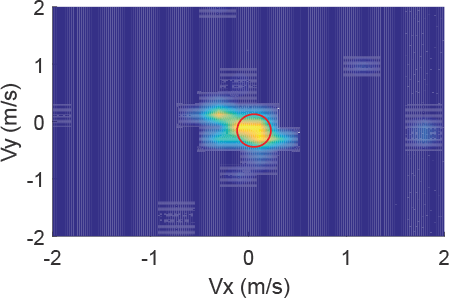
\includegraphics[width=\textwidth]{figures/bvp_stage_1_start}
		\caption{Stage 1: Start}
	\end{subfigure}
	\hfill
	\begin{subfigure}{0.22\textwidth}
		\centering
		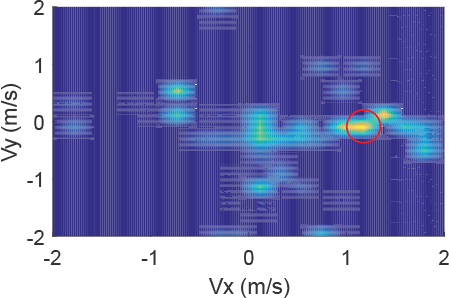
\includegraphics[width=\textwidth]{figures/bvp_stage_2_pushing}
		\caption{Stage 2: Pushing}
	\end{subfigure}
	\hfill
	\begin{subfigure}{0.22\textwidth}
		\centering
		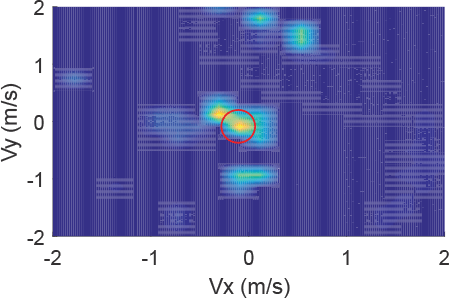
\includegraphics[width=\textwidth]{figures/bvp_stage_3_stop}
		\caption{Stage 3: Stop}
	\end{subfigure}
	\hfill
	\begin{subfigure}{0.22\textwidth}
		\centering
		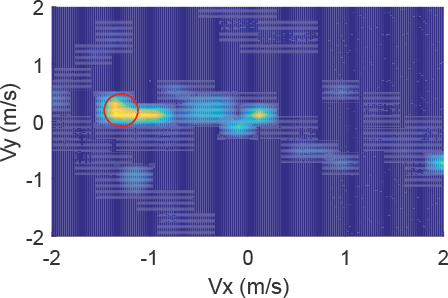
\includegraphics[width=\textwidth]{figures/bvp_stage_4_pulling}
		\caption{Stage 4: Pulling}
	\end{subfigure}
	\caption{A series of slices of a BVP representation of a pushing and pulling gesture, sliced along the time axis. The main velocity component, which represents the movement of the subject's hand, is highlighted with a red circle. This set of images is taken directly from \cite{zheng2019zero}.}
	\label{fig:bvp-example}
\end{figure}

The CSI information, while useful, is also very heavily subjected to various domain factors including, but not limited to, the body composition of the subject, the various objects and their positioning in a room, the direction the subject is facing, the intensity of solar radiation on a given day, and whether Venus is ascending and in Taurus\footnote{The last two were meant as a joke, but is meant to illustrate how difficult it can be to fully characterize all domain factors which may affect the CSI information and how seemingly small things may have alter the CSI signal entirely}.
To remedy this, Zheng et al. \cite{zheng2019zero} proposes the use of the Body-coordinate Velocity Profile (BVP), a representation of the CSI which is theoretically independent of domain factors \cite{zheng2019zero}.
A visual representation of BVP can be seen in Figure \ref{fig:bvp-example}.

BVP is derived through a multi-step process where the CSI is first analyzed to capture both the Doppler Frame Shift (DFS) information and to estimate orientation and location of the subject.
The DFS $D$ is then a matrix with dimensions $F \times M$ where $F$ is the number of sampling points in the frequency domain, i.e., the channels, and $M$ the number of transceiver pairs.
The full derivation of DFS from CSI can be seen in Equation 2 of \cite{zheng2019zero}.

The BVP $V$ is derived from the DFS as a discrete $N \times N$ matrix with $N$ being the number of possible values of velocity components decomposed along each axis of the body coordinates.
The authors of \cite{zheng2019zero} use the local body coordinates of the subjects as the origin with the positive x-axis aligning with the orientation of the person.
The full details of the BVP derivation, which are somewhat unnecessary to the understanding of the rest of this thesis, can be found in Section 4 of \cite{zheng2019zero}.

Suffice to say, the BVP representation of a gesture is an $N \times N \times T$ tensor, where $T$ is the time dimension.
This BVP is thus representative of dynamic effects brought by movement of the subject in the DFS representation of the CSI signal and aligned to the orientation and centered on the location of the subject.

\section{Signal-to-Image Transformations}\label{sec:background-signal-to-image}

In this section, we will look into the mathematical formulation of GAFs, MTFs, and RPs and provide a brief overview of how each of these methods transform a time-series data signal into a tensor which can be interpreted as an image.

\subsection{Gramian Angular Fields}

GAFs \cite{wang2015imaging} represents time series in a polar coordinate system and plots the angles in this system.

First, let $X$ be the input signal of length $n$ and $\tilde{X}$ the input rescaled to the interval $[-1, 1]$.

We then represent $\tilde{X}$ in polar coordinates with arguments for the angle $\phi$ and radius $r$ as

\begin{equation}
	\begin{cases}
		\phi = \arccos(\tilde{x}_i), & \tilde{x}_i \in \tilde{X} \\
		r = \frac{t_i}{N}, & t_{i} \in \mathbb{N}
	\end{cases}
\end{equation}
where $t_{i}$ is the timestamp of a given value of $x_i$ and $N$ a constant factor to regularize the span of the polar coordinates.

This is then transformed into the matrix $G$ of size $n \times n$ as

\begin{align}
	G &= \begin{Bmatrix}
		\cos(\phi_1 + \phi_1) & \cdots & \cos(\phi_1 + \phi_n) \\
		\cos(\phi_2 + \phi_1) & \cdots & \cos(\phi_2 + \phi_n) \\
		\vdots                & \ddots & \vdots \\
		\cos(\phi_n + \phi_1) & \cdots & \cos(\phi_n + \phi_n)
	\end{Bmatrix}
	&= \tilde{X}' \cdot \tilde{X} - \sqrt{I - \tilde{X}^2}' \cdot \sqrt{I - \tilde{X}^2}
\end{align}
where $I$ is the unit row vector $[1, 1, \ldots, 1]$.
Defining the inner product $< x,y> = x \cdot y - \sqrt{1 - x^2} \cdot \sqrt{1-y^2}$ results in G being a Gramian matrix with
\begin{equation}
	G = \begin{Bmatrix}
		< \tilde{x}_1, \tilde{x}_1 > & \cdots & < \tilde{x}_1, \tilde{x}_n >\\
		< \tilde{x}_2, \tilde{x}_1 > & \cdots & < \tilde{x}_2, \tilde{x}_n > \\
		\vdots                       & \ddots & \vdots \\
		< \tilde{x}_n \tilde{x}_1 > & \cdots & < \tilde{x}_n, \tilde{x}_n >
	\end{Bmatrix}
\end{equation}

The GAF provides a way to preserve temporal dependencies, with time increasing along the diagonal from the top left to the bottom right.

\subsection{Markov Transition Fields}

MTFs \cite{wang2015imaging} encode the dynamical transition statistics of a time series by representing these transitions as Markov transition probabilities.
Let the input signal $X$ of length $n$ be quantized into $Q$ bins.
Each sample $x_i$ from the input signal is then placed in the corresponding bin $q_j, j \in [1, Q]$.
A matrix $M$ of size $n \times n$ is then constructed where $M_{ij}$ denotes the probability of a transition between bins $q_i \rightarrow q_j$ between two sequential time steps. 
Let the quantile bins that contain the data at timestep $i$ and $j$ be $q_k$ and $q_l$, respectively.
This formally defines $M$ as
\begin{equation}
	M = \begin{Bmatrix}
			w_{kl|x_1 \in q_k, x_1 \in q_l} & \cdots & w_{kl|x_1 \in q_k, x_n \in q_l} \\
			w_{kl|x_2 \in q_k, x_1 \in q_l} & \cdots & w_{kl|x_2 \in q_k, x_n \in q_l} \\
			\vdots                          & \ddots & \vdots                          \\
			w_{kl|x_n \in q_k, x_1 \in q_l} & \cdots & w_{kl|x_n \in q_k, x_n \in q_l}
		\end{Bmatrix}
\end{equation}
$M$ is then an image of size $n \times n$ and can be interpreted as representing the probabilities of any state transitioning into another state over time.

\subsection{Recurrence Plots}

RPs \cite{eckmann1995recurrence} transform the image by representing distances between extracted trajectories in the original time series.
Let the input signal $X$ of length $n$ have extracted trajectories
\begin{equation}
	\vec{x}_i = \left(x_i, x_{i+\tau},\ldots, x_{i+(m-1)\tau}\right), ~ \forall i \ in \{1,\ldots,n-(m-1)\tau\}
\end{equation}
where $m$ is the dimension of the trajectories and $\tau$ is the time delay.
We can then construct the recurrence plot $R$ as the a matrix of size $\left(n - (m-1)\tau\right) \times \left(n - (m-1)\tau\right)$.
Every value in this matrix is defined as the pairwise distance between trajectories, formally
\begin{equation}
	R_{i,j} = \Theta\left(\epsilon - ||\vec{x}_i - \vec{x}_j|| \right),~\forall i,j \in \{1, \ldots, n-(m-1)\tau\}
\end{equation}
where $\epsilon$ is a threshold and $\Theta$ is the Heaviside function given by
\begin{equation}
	\Theta(x) := \begin{cases}
		1, & x \geq 0\\
		0, & x < 0
	\end{cases}
\end{equation}

This can be interpreted as representing the pairwise distance between trajectories which are above a certain threshold.

\chapter{Methodology}\label{chapter:methodology}

\begin{figure}
	\centering
	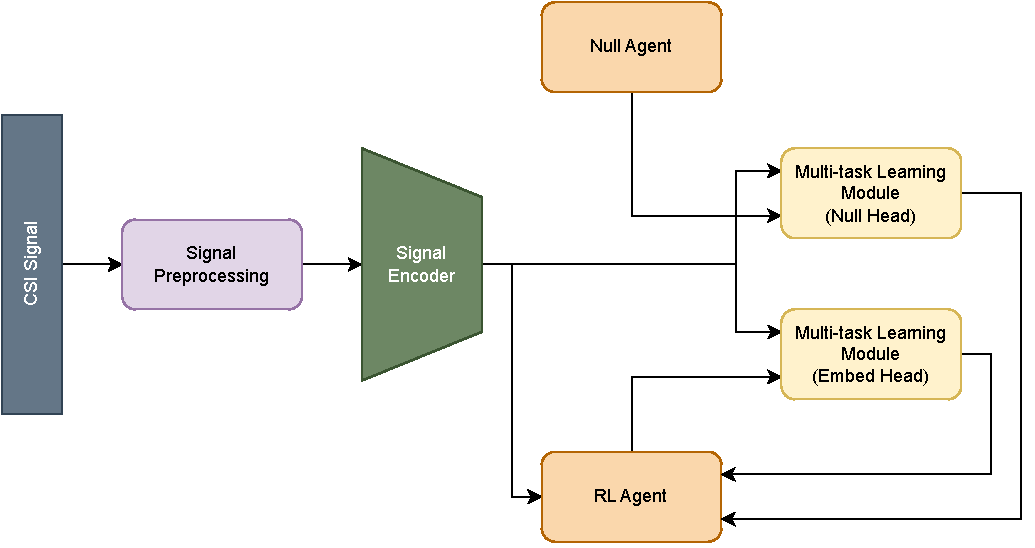
\includegraphics[width=\linewidth]{figures/arch_diagram.pdf}
	\caption{An abstracted diagram of the proposed DARLInG architecture.}
	\label{fig:arch-diagram}
\end{figure}

This chapter will first discuss the details of the dataset which we are using. 
We will discuss our approach to the problem of domain agnostic Wi-Fi CSI gesture classification and delve into the details of our chosen architecture.
This will first begin with a general overview of our method, then discuss each component of the architecture individually as well as their motivations and intuitions.

\section{Widar 3.0}

\begin{figure}
	\centering
	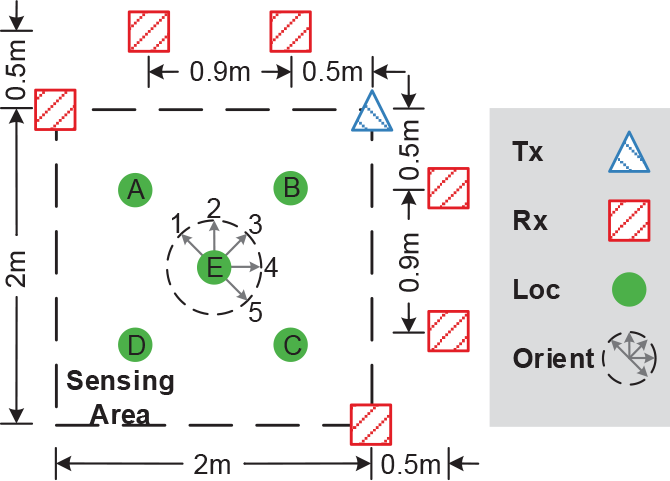
\includegraphics{figures/widar-positioning}
	\caption{Typical positioning of the access points and subjects in Widar. The image is sourced from \cite{zheng2019zero}. Loc shows the different torso locations used and orient the different orientations the subject may be at.}
	\label{fig:widar-positioning}
\end{figure}

Widar\cite{zheng2019zero} contains gesture data collected over a series of months in 3 different rooms with 17 different subjects.
6 gestures were performed by every subject.
For each gesture performed, the gesture was performed in one of 5 locations with 5 orientations.
Further details of the distribution of domain factors can be found in Appendix \ref{appendix:dataset}.
Further details of how the data was gathered can be found in \cite{zheng2019zero}.

Each recorded data sample is a time-series consisting of the CSI between a transmitting Wi-Fi access point (Tx) and a receiving Wi-Fi access point (Rx).
Each Rx access point (AP) has two antennas, each of which are collecting separate time-series streams.
The positional setup of the gesture collection spaces can be seen in Figure \ref{fig:widar-positioning}.

The data itself is provided as a collection of both CSI data dumps, collected at 1000 Hz, as well as BVP tensors, collected with a temporal resolution of 10 Hz.
Each CSI data dump contains samples of sets of complex values with variable length, the shortest having a length of around 100 samples and the longest with a length of around 3100 samples. 
As the majority of the data have a length of less than 2000 samples, we set the cutoff to 2000 samples to ensure that every datapoint we use for training has the same length. 
We pad those of shorter length with 0s and we simply apply a cutoff on those datapoints which are longer.

Due to our focus on looking at single domain factor leave out as our main research question, we have chosen the task of single-user leave out.
To ensure that we are focusing only on this domain factor, our selection parameters for the training set and test set are seen in Table \ref{tab:single-user-select}.

\section{DARLInG}

In this thesis, we present our novel approach DARLInG (Domain Autolabeling through Reinforcement Learning for the Identification of Gestures).
DARLInG is our proposed approach to domain-independent gesture identification using RL.
Our intuition comes from \cite{zhang2021adversarial} in which RL was used to identify features in the data which was invariant to domain shifts.
Analogously, we hypothesize that RL can then be used to identify those features which are \textit{not} invariant to domain shifts and produce a \textit{domain embedding} from said features.
We hypothesize that by providing our gesture discriminator with not only the original signal, encoded by a CNN-based VAE encoder, but also this domain embedding, the gesture discriminator would be able to significantly increase its performance in gesture recognition throughout multiple domains.

The general architecture of DARLInG can be seen in Figure \ref{fig:arch-diagram} and the code can be found publicly on GitHub\footnote{\href{https://github.com/yvan674/DARLInG}{https://github.com/yvan674/DARLInG}}.
We first propose a signal processing and signal-to-image transformation pipeline, described in Section \ref{sec:methodology-signal-preprocessing}.
This transforms the input signal into an image that is then passed through a CNN encoder, as described in Section \ref{sec:methodology-signal-encoding}, encoding the signal into a latent space.
This latent representation is then used in two different ways: As an input for the multi-task learning heads, described in Section \ref{sec:methodology-multi-task-learning}, and as the state observation for our RL agent, described in Section \ref{sec:methodology-rl}.

\begin{figure}
	\centering
	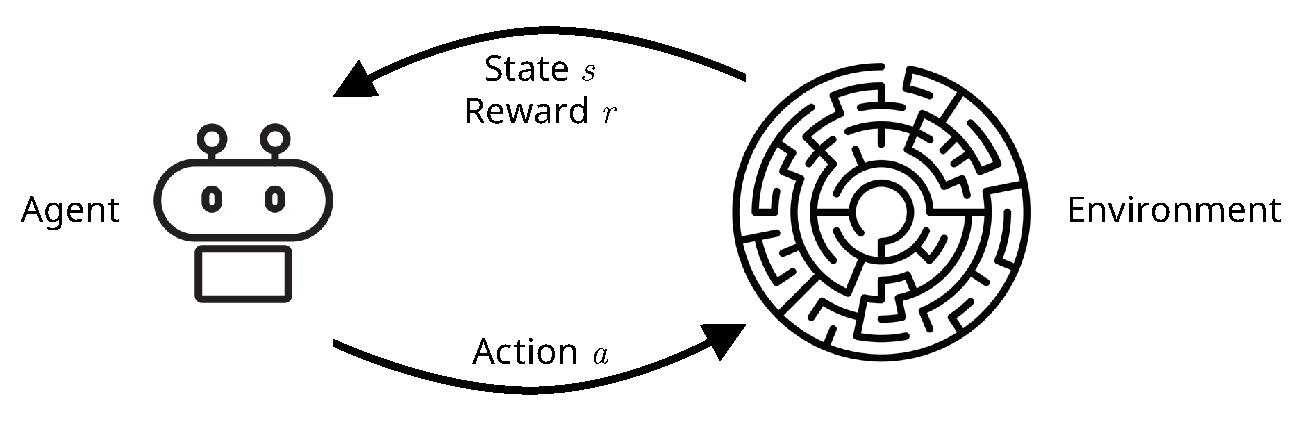
\includegraphics[width=0.78\textwidth]{figures/rl_paradigm}
	\caption{The basic paradigm of Reinforcement Learning where an agent interacts with its environment through actions $a$ and receives a new state $s$ and reward $r$ in return.}\label{fig:rl-paradigm}
\end{figure}
Recall first that RL is typically modeled as a Markov decision process with an environment and observed state $s_t$ of said environment at time $t$.
An agent then performs an action $a_t$ and is provided with a reward $r_t$ and a new observed state $s_{t+1}$.
A typical RL scenario is framed in this way and is visually represented by Figure \ref{fig:rl-paradigm}.

To mitigate domain-shift, our RL agent is tasked with producing the best possible domain embedding of the domain $\boldsymbol{d}_r = a, \boldsymbol{d}_r \in [0, 1]^e$ as its action where $e$ is the dimensionality of the domain embedding.
The domain embedding, or action, is generated by the RL agent given the signal latent representation $\boldsymbol{z} = s, \boldsymbol{z} \in [0, 1]^f$ as its state observation, where $f$ is the dimensionality of the latent representation.

To provide the RL agent with a reward function we use two different multi-task learning modules.
The details of the reward function are described in Subsection \ref{subsec:methodology-reward}.
One of these modules is provided $\boldsymbol{d}_{\emptyset}$, representing a vector of zeros when $\boldsymbol{d}_r$ is one-hot encoded or a value of $\frac{1}{f}$ when $\boldsymbol{d}_r$ is a probability measure.
The other module is provided with $\boldsymbol{d}_{r} = a$.

\section{Signal Preprocessing}\label{sec:methodology-signal-preprocessing}

\begin{figure}
	\centering
	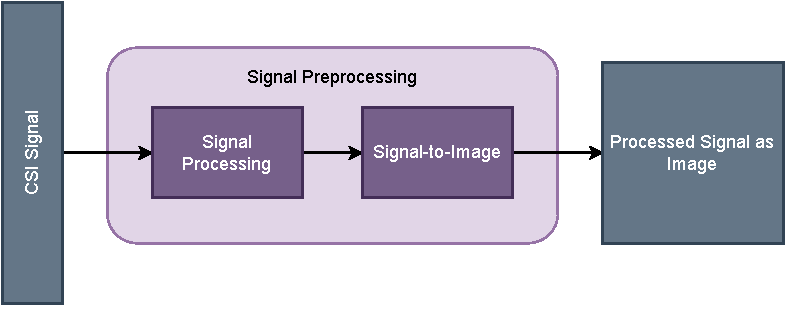
\includegraphics[width=0.8\linewidth]{figures/signal_preprocessing_diagram.pdf}
	\caption{Details of the signal preprocessing module. The module is comprised of traditional signal preprocessing and a signal-to-image transformation.}
	\label{fig:signal-preprocessing-diagram}
\end{figure}

As the old adage goes, garbage in, garbage out.
As such, we propose a signal preprocessing module, visualized in Figure \ref{fig:signal-preprocessing-diagram}.
This module first cleans the CSI signal using traditional signal processing and then transforms it into an image for use by the signal encoder.

\subsection{Signal Processing}

\begin{figure}
	\centering
	\begin{subfigure}{0.49\textwidth}
		\centering
		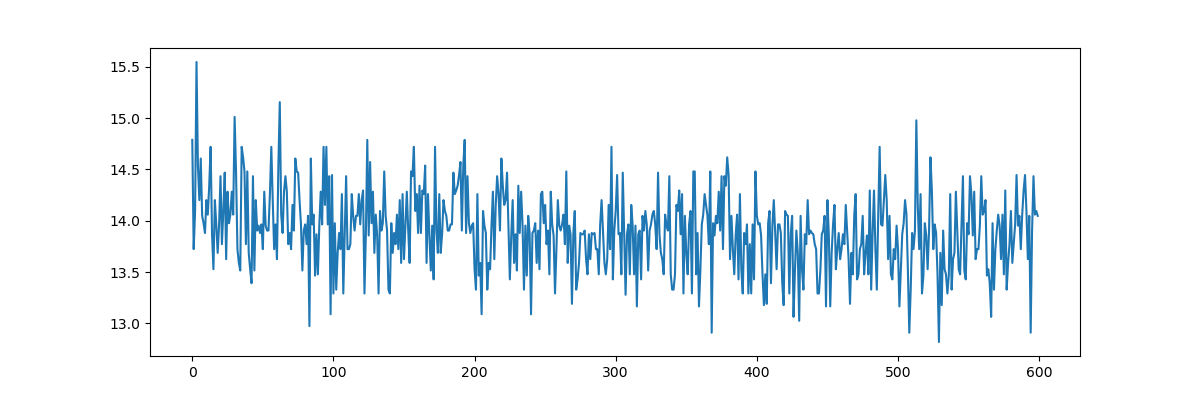
\includegraphics[width=\textwidth]{figures/amp_original}
		\caption{The original amplitude signal.}
	\end{subfigure}
	\hfill
	\begin{subfigure}{0.49\textwidth}
		\centering
		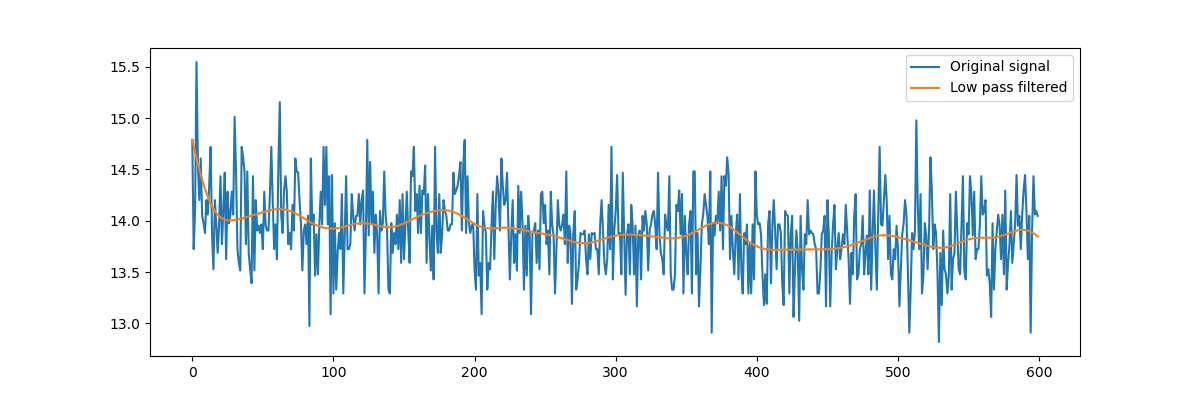
\includegraphics[width=\textwidth]{figures/amp_step_1}
		\caption{The original amplitude signal and the low pass filtered signal.}
	\end{subfigure}
	\hfill
	\begin{subfigure}{0.49\textwidth}
		\centering
		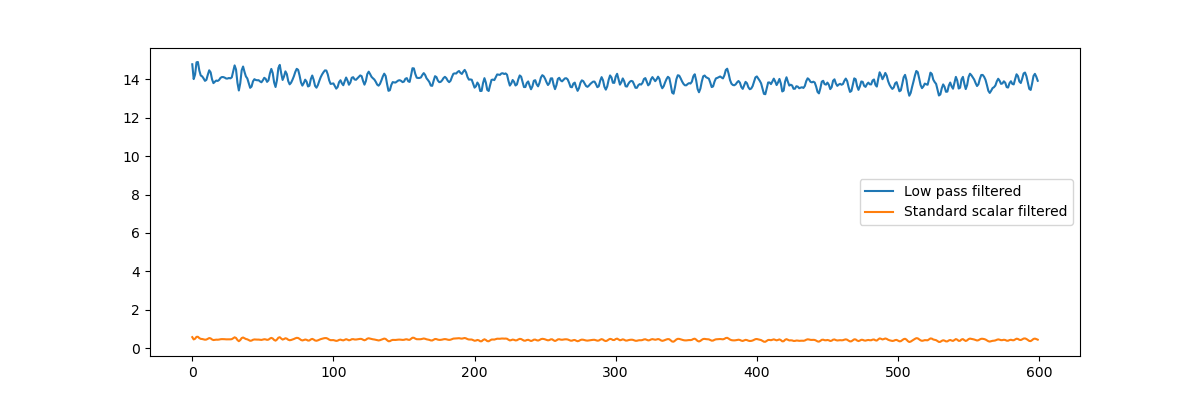
\includegraphics[width=\textwidth]{figures/amp_step_2}
		\caption{The low pass filtered signal and the signal after the standard scalar.}
	\end{subfigure}
	\hfill
	\caption{An example of the amplitude shift signal after being transformed by each step of the signal processing pipeline. Only the first 600 samples of one channel from one tranceiver link is shown here for illustrative purposes.} \label{fig:amp-pipeline}
\end{figure}

\begin{figure}
	\centering
	\begin{subfigure}{0.49\textwidth}
		\centering
		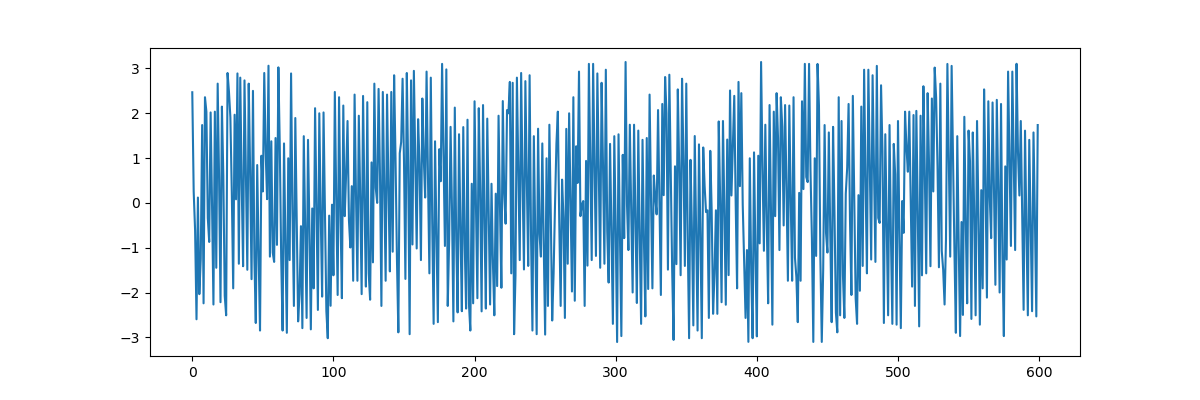
\includegraphics[width=\textwidth]{figures/phase_original}
		\caption{The original phase signal.}
	\end{subfigure}
	\hfill
	\begin{subfigure}{0.49\textwidth}
		\centering
		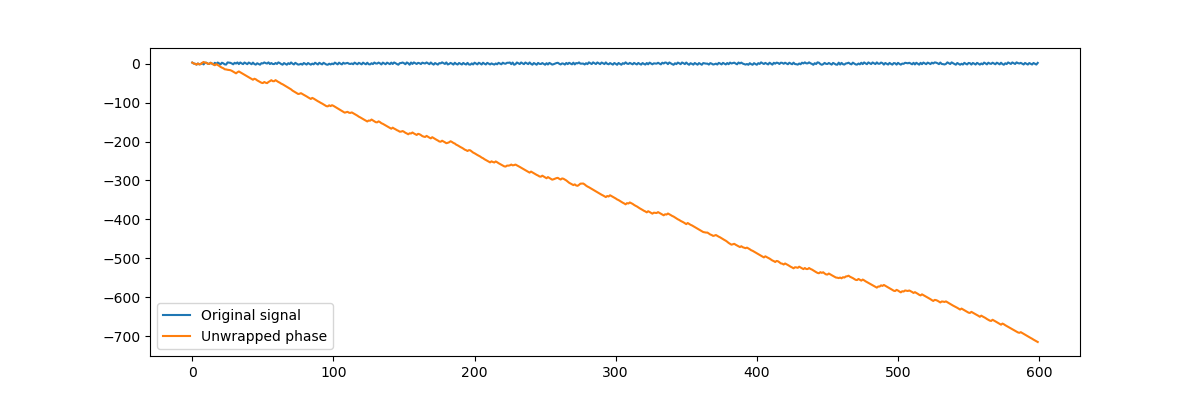
\includegraphics[width=\textwidth]{figures/phase_step_1}
		\caption{The original phase signal and the phase unwrapped signal.}
	\end{subfigure}
	\hfill
	\begin{subfigure}{0.49\textwidth}
		\centering
		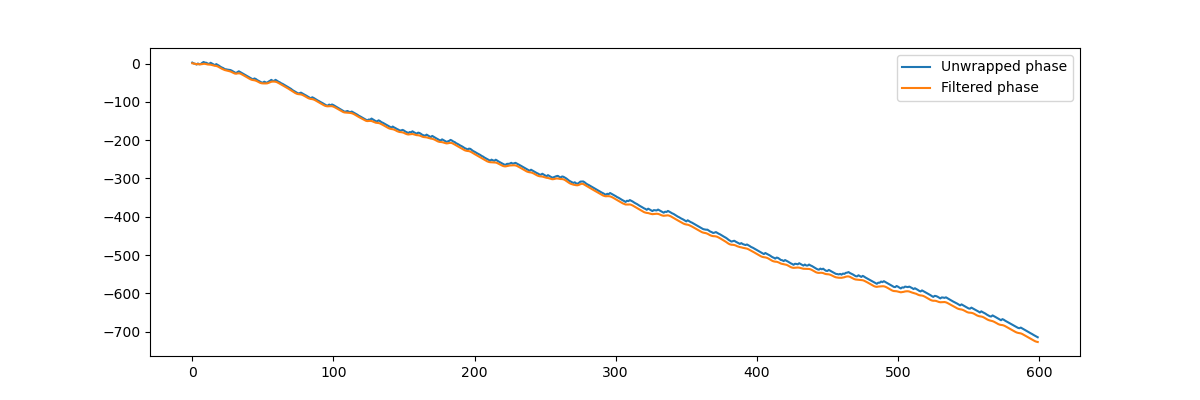
\includegraphics[width=\textwidth]{figures/phase_step_2}
		\caption{The phase unwrapped signal and the phase filtered signal.}
	\end{subfigure}
	\hfill
	\begin{subfigure}{0.49\textwidth}
		\centering
		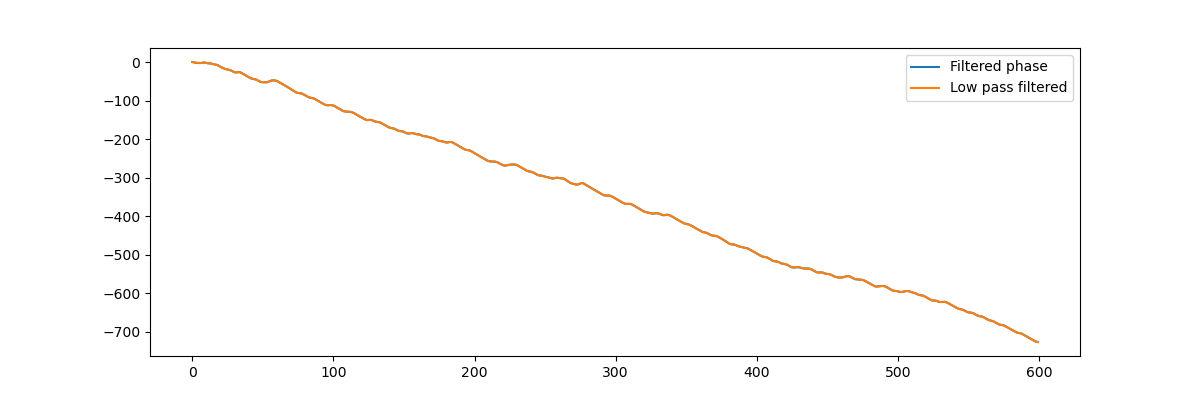
\includegraphics[width=\textwidth]{figures/phase_step_3}
		\caption{The phase filtered signal and the low pass filtered signal.}
	\end{subfigure}
	\hfill
	\begin{subfigure}{0.49\textwidth}
		\centering
		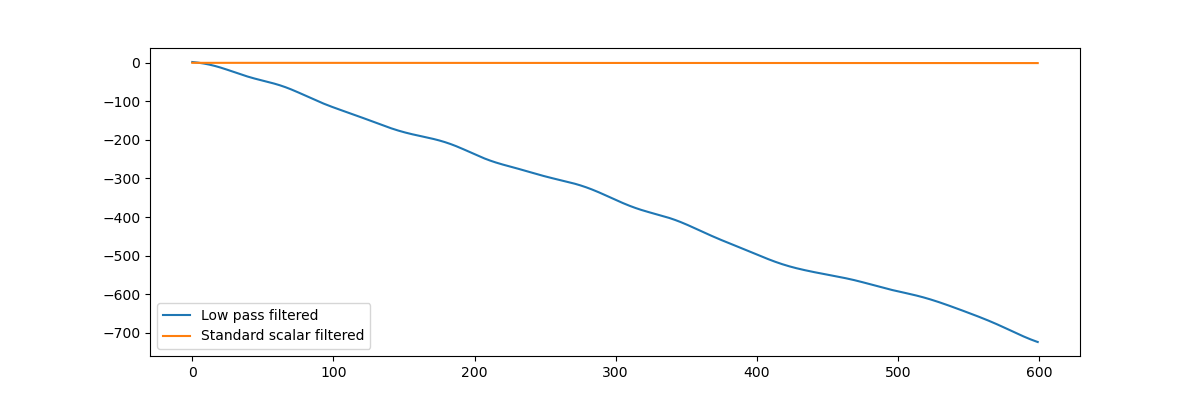
\includegraphics[width=\textwidth]{figures/phase_step_4}
		\caption{The low pass filtered signal and the signal after the standard scalar.}
	\end{subfigure}
	\hfill
	\caption{An example of the phase shift signal after being transformed by each step of the signal processing pipeline. Only the first 600 samples of one channel from one tranceiver link is shown here for illustrative purposes.} \label{fig:phase-pipeline}
\end{figure}

\begin{figure}
	\centering
	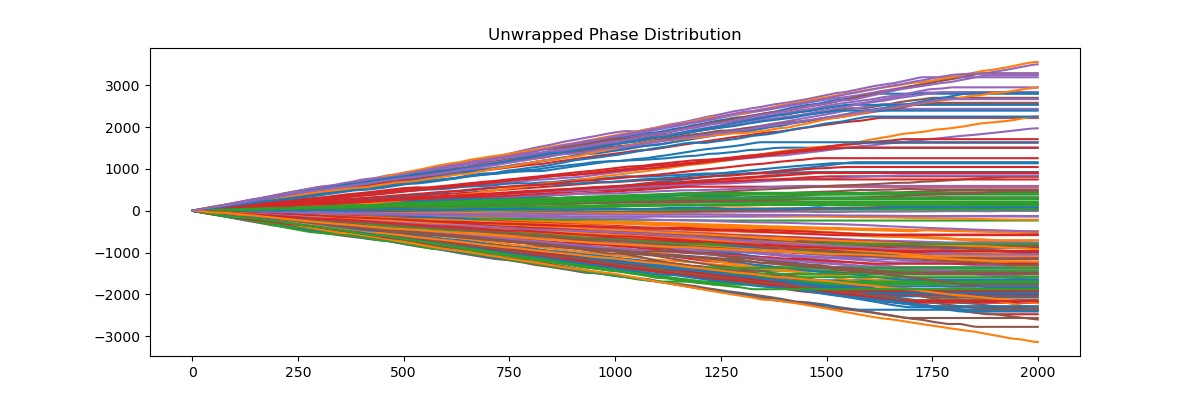
\includegraphics[width=0.8\textwidth]{figures/phase_unwrap}
	\caption{A plot over time of the phase shift after unwrapping of all training data, colored by gesture, showing how there is no general trend of only increasing or decreasing phases. A histogram shows the final phase unwrapped values. The histogram shows the final values are generally positive, but tend to not be at the extremes.}\label{fig:phase-unwrap}
\end{figure}

The CSI data is provided as a set of complex values sampled at 1000 Hz.
We first decompose this into its radius and angle components on the complex plane.
These correspond to the amplitude and phase shift of the signal, respectively.
We process this signal through two different pipelines, one for the amplitude component and one for the phase component, as the phase requires a few additional processing steps compared to the amplitude.

The pipeline for amplitude consists of the following steps:

\begin{enumerate}
	\item \textbf{Low Pass Filter} set to a cutoff frequency of 250 Hz and an order of 4.
	\item \textbf{Standard Scalar} which has been trained on all training data and transforms the signal to have a mean of 0 and a standard deviation of 1.
\end{enumerate}

The low pass filter is used to eliminate noise inherent in CSI data from environmental factors.
It has been set to these values based on empirical experimentation which shows that no human movements during the performance of the 6 gestures which we test for has a frequency above 250 Hz.

The standard scalar is used since empirical evidence shows that neural networks work best when input values are close to the interval $[-1, 1]$ \cite{varun2023tuning}.
The standard scalar we use is fitted on the training set of the split that is used during a given experiment.

The effect of each step of the amplitude pipeline can be seen in Figure \ref{fig:amp-pipeline}.

The pipeline for the phase consists of the following steps prepended to the amplitude pipeline:
\begin{enumerate}
	\item \textbf{Phase Unwrapping} which unwraps the phase and makes the signal continuous.
	\item \textbf{Phase Filtering} step, which applies a uniform and median filter onto the phase shift signal.
\end{enumerate}

We use phase unwrapping to avoid sharp discontinuities in the phase value whenever a phase wraps around from $-\pi$ to $\pi$ or vice versa.
This results in a continuous signal instead of disjointed segments of the signal.
We use phase filtering as inspired by \cite{oerlemans2022effect} with the same parameters and for the same reasons.
The effect of each step of the phase pipeline can be seen in Figure \ref{fig:phase-pipeline}.

The signal can now be considered clean, or at least clean enough that we can continue with further steps.

During the course of experimentation, we considered taking the derivative of the phase, to eliminate a generally monotonously increasing or decreasing signal, as can been seen in the example in \ref{fig:phase-pipeline} after phase unwrapping.
Further investigation showed that this is not necessary as most signals do not monotonously increase or decrease.
A plot of the phase shifts after unwrapping of all signals can be seen in Figure \ref{fig:phase-unwrap}.
The plot clearly shows that there is no general trend of phases increasing or decreasing infinitely, with many phase shifts staying slightly positive after unwrapping but few signals trending towards the extreme ends of the distribution.

\subsection{Signal-to-Image Transformation}\label{sec:methodology-signal-to-image}
\begin{figure}
	\centering
	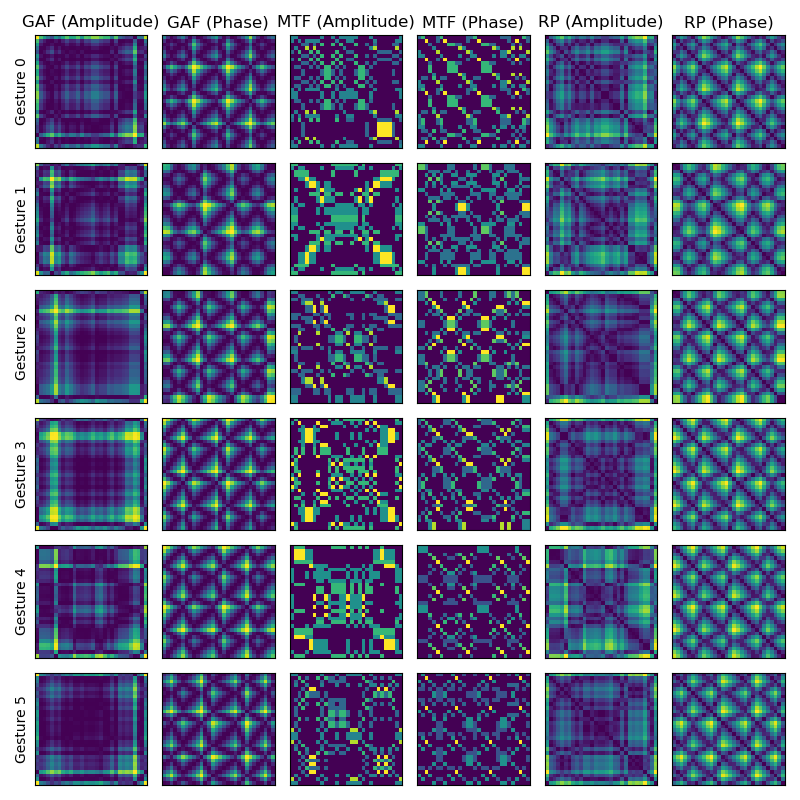
\includegraphics[width=\textwidth]{figures/transforms}
	\caption{Samples of each gesture from Widar being transformed using each of the three signal-to-image transformations. Each pair of columns is the transformation by a single signal-to-image transformations on the amplitude and phase signals, respectively.}
	\label{fig:transform-samples}
\end{figure}

%Four crazy signal-to-image transformation methods! You won't believe number three!\todo{If there are no objections, this will be in the final paper}

The next stage in our method is transform the signal into an image, leveraging advances from computer vision.
We will experiment with the following three methods for signal-to-image transformation: Gramian Angular Fields (GAF) \cite{wang2015imaging}, Markov Transition Fields (MTF) \cite{wang2015imaging}, and Recurrent Plots (RP) \cite{eckmann1995recurrence}.
A more comprehensive description of each of these transformations can be found in Section \ref{sec:background-signal-to-image}.

We process these images in Python using the pyts package \cite{faouzi2020pyts} which conveniently contains ready-to-use implementations of all three of the aforementioned transformations.
Regardless of the chosen transformation, the signal is transformed into a two-dimensional tensor which can be treated as an image.
We also downsample this image to a size of $40 \times 40$ pixels for computational complexity purposes, which still provides a temporal resolution $4 \times$ that of the provided BVP data in Widar.
A visualization of each of the signal-to-image transformations on randomly selected samples of the Widar 3.0 dataset can be seen in Figure \ref{fig:transform-samples}.
As can be seen, each CSI sample is transformed into an amplitude as well as a phase image.
We can then proceed with the encoding of this image into a latent space.

\section{Signal encoding}\label{sec:methodology-signal-encoding}

\begin{figure}
	\centering
	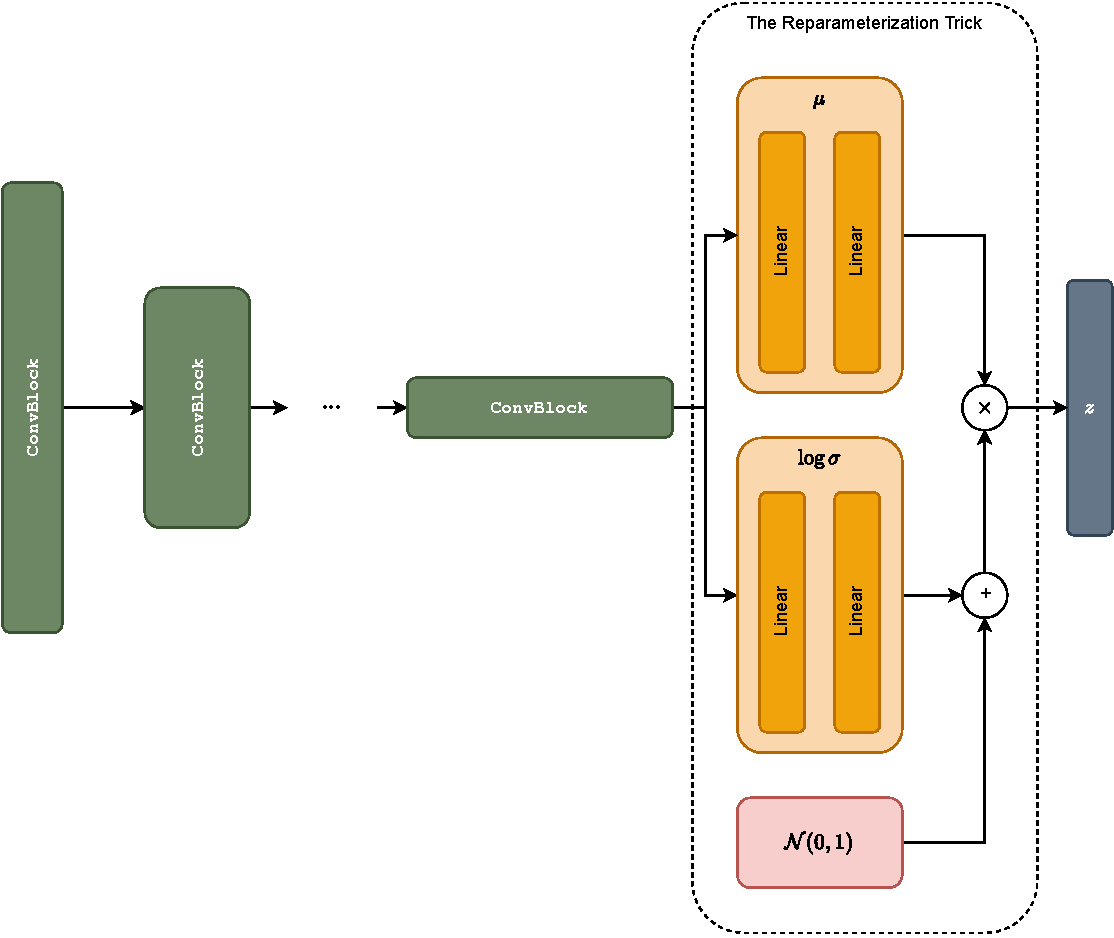
\includegraphics[width=\textwidth]{figures/vae-diagram}
	\caption{The CNN-based VAE used in DARLInG. The number of ConvBlock elements is variable, depending on the experiment being performed. The reparameterization trick is described in \cite{kingma2013auto}.}\label{fig:vae-diagram}
\end{figure}

The encoding of the signal, now an image, into a latent space is performed using a Convolutional Neural Network (CNN)-based VAE.
The CNN itself is structured as a standard, deep CNN, made up of multiple \verb|ConvBlock|s where each block is made up of a \verb|Conv2d| with dropout, a batch norm layer, and an activation layer.
The number of input channels, filters, and kernel size of the 2-D convolutional layer and its dropout is set dynamically and differs by experiment.
The activation function also differs by experiments and is either ReLU, LeakyReLU, or SeLU.
The number of \verb|ConvBlock|s is set dynamically and differs by experiment.

These blocks are then followed by two sets of two fully connected layers with a hidden layer size of 8192.
One set of these fully connected layers serve to predict the $\mu$ and the other set to predict the $\log \sigma$ of the latent variables.
The reparameterization trick is then used, adding a random variable $\mathcal{N}(0, 1)$ to produce the latent variables $\boldsymbol{z}$.
A visualization of the CNN-based VAE used can be seen in Figure \ref{fig:vae-diagram}.

The latent representation $\boldsymbol{z}$ of this signal is then passed to both the reinforcement learning agent as its state observation as well as to the multi-task learning modules.

In the case of CSI data, as the signal is provided as both an amplitude and phase image, we have two signal-encoding modules running in parallel; one for the amplitude image and one for the phase image with no sharing of parameters.
How the RL agent uses this state observation is described in Section \ref{sec:methodology-rl} while its use by the multi-task learning module is described in Section \ref{sec:methodology-multi-task-learning}.

\section{Multi-task Learning}\label{sec:methodology-multi-task-learning}

\begin{figure}
	\centering
	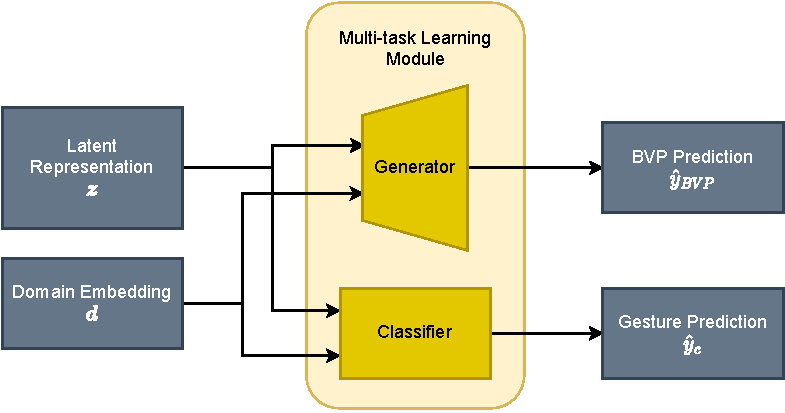
\includegraphics[width=0.8\linewidth]{figures/multitask_learning_module_diagram.pdf}
	\caption{Details of the multi-task learning module. The generator is made up of a series of deconvolutional layers and produces the BVP prediction while the classifier is a fully connected network and produces a probability distribution over each gesture class.}
	\label{fig:multitask-learning-module-diagram}
\end{figure}

The actual gesture classification module is built using a multi-task learning module, a visualization of which can be seen in Figure \ref{fig:multitask-learning-module-diagram}.
The idea, intuitively, is to enforce some sort of representation that is already approaching a domain-invariant representation of the data.
To do so, we use the generation of the BVP as an auxiliary task while keeping gesture recognition as our main task.
This is done as BVP is theoretically domain-independent \cite{zheng2019zero}, even though we are ultimately not interested in the BVP.
This approach is inspired by Martini et al. \cite{martini2021domain}, which, although using a different metric to modulate domain-independence as an optimization objective, suggests that an adversarial approach modulating both a domain-independence objective and a domain-discrimination objective can be powerful and increase classification performance.
The BVP generation is done by a series of deconvolutional layers while the classifier is a series of fully-connected layers.
Additionally, it has been shown empirically that multi-task learning can produce better results in each target task as opposed to dedicated networks \cite{tuggener2021deepscoresv2}.
This is likely due to the encoder being guided towards producing a more robust or efficient latent representation capable of being used for many different tasks instead of a latent representation focused on only one task.

Therefore, as BVP generation is a theoretically domain-independent process, we should expect the latent representation to contain both features which are completely domain independent as well as features which are not.
We do not, however, want to enforce domain-independence directly on the latent representation, as this may result in worse performance \cite{van2022insights}.

As seen in Figure \ref{fig:arch-diagram}, we utilize two multi-task learning modules. The module receiving $\boldsymbol{d}_\emptyset$ is termed the \textit{null head} while the module receiving $\boldsymbol{d}_r$ is termed the \textit{embed head}. 
The motivation behind the use of two heads is such that we can measure the RL agent's performance in an unsupervised manner by comparing the performance of the null head to the embed head.
Intuitively, we should expect the embed head to perform better if the embedding $\boldsymbol{d}_r$ provided by the RL agent is able to provide some useful information, likely with respect to the domain, as opposed to the null head, which receives no useful information.

For the loss function, we use cross entropy loss on the gesture classifier and mean squared error loss on the BVP generation.

\section{Reinforcement Learning Agent}\label{sec:methodology-rl}

To mitigate domain shift, we implement a novel method for unsupervised domain autolabeling through reinforcement learning.
Recall the common terminology used in RL, the agent, the action $a$, the state observation $s$, the reward $r$, and the learning paradigms discussed in Section \ref{sec:background-rl}.
For our agent, we choose to use the output of the encoder $\boldsymbol{z}$ as its state observation $s$.
The agent then performs an action $a$ which is what we refer to as the domain embedding $\boldsymbol{d}_r$.
This domain embedding is either continuous, in the case where the $\boldsymbol{d}_r$ is understood as a probability measure, or discrete, in the case where the $\boldsymbol{d}_r$ is understood as a one-hot encoding of domain factors.
The produced $\boldsymbol{d}_r$ is then concatenated to one copy of $\boldsymbol{z}$ and fed to the embed head, while the other head receives a copy of $\boldsymbol{z}$ concatenated with $\boldsymbol{d}_\emptyset$.
The reward $r$ is produced as a function of the outputs of both heads, and will be discussed further in Subsection \ref{subsec:methodology-reward}.

In this work, we will be looking at using both PPO and DDPG, on-policy and off-policy algorithms, respectively.
Details of PPO can be found in Subsection \ref{subsec:background-ppo} while the details of DDPG can be found in Subsection \ref{subsec:background-ddpg}.
We use the ready-to-use implementation from Stable Baselines 3 \cite{raffin2021stable}, which also requires interpreting the model itself as a Gymnasium environment.
Gymnasium is an open-source RL framework previously mainted by OpenAI, but now actively maintained by the Farama Foundation \cite{towers2023gymnasium}.

Our use of RL to tackle this problem is inspired by both \cite{ma2021location} and \cite{zhang2021adversarial}.
In \cite{ma2021location}, as discussed in Section \ref{sec:literature-csi-for-gesture}, RL was successfully used to eliminate the need for domain-specific information Wi-Fi CSI gesture recognition.
On the other hand, as discussed in Section \ref{sec:literature-domain-rl}, \cite{zhang2021adversarial} used RL for domain-independent feature selection.
We therefore were motivated to investigate whether RL could also be used to perform the opposite: to extract relevant domain-specific features and produce a useful embedding of said features for gesture recognition.

\subsection{Known Domain Encoding}
We also used a ``known'' domain encoding as our baseline.
This is a 33-dimensional one-hot encoding of the known domain factors (i.e., twenty users, three room, five face orientations, and five torso locations).
For example, in the case of user 2 in room 1 with face orientation 4 and torso location 3, the known domain embedding would be
\begin{align*}
	\boldsymbol{d}_r = [&0,1,0,0,0,0,0,0,0,0,0,0,0,0,0,0,0,0,0,0 & \text{user encoding} \\
	                    &1,0,0                                   & \text{room encoding} \\
	                    &0,0,0,1,0                               & \text{orientation encoding} \\
	                    &0,0,1,0,0]                              & \text{location encoding}
\end{align*}

This was used as a baseline to compare our RL agents against.
The intuition behind this is that our initial hypothesis is essentially ``providing domain labels can increase model performance''.
Therefore, the known domain factors, while incomplete, should provide \textit{some} baseline to which we can compare our model again.
We do not need a specific baseline of a model with no domain labels since this is already incorporated into our algorithm in the form of the null head.

\subsection{Reward Function}\label{subsec:methodology-reward}

As with any RL algorithm, one of the most important components is the reward function used.
We experiment with two different reward functions: One we call the \textit{contrastive reward} $R_{CON}$ and one we call \textit{distance-maximization contrastive reward} $R_{DMC}$.

\paragraph{Contrastive reward}
Let $\varrho$ denote some metric subject to minimization to measure the gesture classification performance of a multi-task learning module given the gesture classification prediction $\hat{y_{c}}$.
The contrastive reward function $R_{CON}$ is then 
\begin{equation}
	R_{CON}(\hat{y}_{c,r}, \hat{y}_{c,\emptyset}, y_c, \gamma) = \gamma \cdot \left(\varrho\left(\hat{y}_{c,\emptyset} - y_c\right(\phi\left(\hat{y}_{c,r}, y_c\right))\right)
\end{equation}
where $y_c$ is the ground truth gesture classification, $\hat{y}_{c,r} $ the predicted gesture from the embed head, $\hat{y}_{c,\emptyset}$ the predicted gesture from the null head, and $\gamma$ a multiplier factor chosen during hyperparameter tuning.
In practice, we use cross entropy loss as our performance metric $\varrho$.
As such, our reward function $R_{CON}$ calculates the gesture recognition performance difference between the embed and null heads.

Intuitively, we use this as our metric as the reward is based on the performance difference between the two heads.
As the only difference in inputs between the two heads is that one receives $\boldsymbol{d}_r$ while the other receives $\boldsymbol{d}_\emptyset$, we should expect the difference in performance to come solely out of a difference in how powerful the domain embedding provided by the RL agent is in describing the domain factors influencing the CSI signal.
Thus, maximizing this difference implies better total model performance.
We do not use an absolute value, as we want to penalize the model if the domain embedding results in the embed head performing worse than the null head.

This reward can be thought of as being similar to testing the null hypothesis, where $H_0$ is provided by the null head and $H_1$ is provided by the embed head.
Our hypothesis, that the domain embedding will provide better results, is measured by the performance difference between then null and embed head, by proxy.
If the RL agent provides a useful domain embedding, then the reward will approach $\gamma \cdot \varrho\left(\hat{y}_{c,\emptyset}\right)$.

\paragraph{Distance-Maximization Contrastive Reward}
Empirical results show that the contrastive reward was not able to produce good performance.
After inspecting the embeddings provided by our RL agent, we observed that the difference in value between each dimension was quite minimal, i.e., the agent produced results similar to $\boldsymbol{d}_\emptyset$.
We believe this is due to the agent attempting to minimize the penalty for worse performance without being incentivized enough to achieve positive rewards.

In response, we introduce our \textit{distance-maximization contrastive reward} $R_{DMC}$.
With this reward function, we hope to incentivize the agent to produce domain embeddings which are more informative by maximizing the difference between each dimension of the domain embedding.
The idea here is to provide stronger signals for the multi-task heads.
We do this by first calculating the pairwise difference between each of the dimensions.
We then apply a threshold to the difference, where any value below $\alpha$ is zeroed out, similarly to the procedure used in Lasso regression.
Finally, we sum together all differences and divide by the number of non-zero values and add the contrastive loss.
Formally, this is given by
\begin{align}
	R_{DCM} (\hat{y}_{c,r}, \hat{y}_{c,\emptyset}, y_c, \boldsymbol{d}_r, \gamma) &= \gamma \cdot
		\frac{\sum_{i \leq e} \sum_{j \leq e, j > i} \left(|d_{r,i} - d_{r,j}|\right) \cdot \mathds{1}_{>\alpha}\left(|d_{r,i} - d_{r,j}|\right)}
		     {\sum_{i \leq e} \sum_{j \leq e, j > i} \mathds{1}_{>\alpha}\left(|d_{r,i} - d_{r,j}|\right)}
		+ R_{CON}(\hat{y}_{c,r}, \hat{y}_{c,\emptyset}, y_c) \\
	\text{where } \mathds{1}_A(x) &:= \begin{cases}
		1, & x \in A\\
		0, & x \notin A
	\end{cases},
\end{align}
$e$ the dimensionality of the domain embedding $\boldsymbol{d}_r$, $\mathds{1}_{A}(x)$ the characteristic indicator function, and $\alpha$ a hyperparameter to tune.
$d_{r,i}$ can be understood as the magnitude of the $i$-th dimension of the domain embedding.
In practice, we set $\alpha = 0.1$.

\section{Model Training}\label{sec:methodology-training}

The general training process of the model is described in Algorithm \ref{algo:darling-training}.
We set the training of the RL agent to begin only at epoch $\zeta$ to ensure that the latent representation provided by the encoder has somewhat stabilized and actually contains useful information.
Otherwise, the RL agent will be training on garbage observation states.
This is especially relevant for DDPG, as the replay buffer may contain observations from those garbage environment states even during the later stages of training.
We alternate training between the RL agent and the VAE, rather than training both simultaneously, as we believe this will lead to more stable performance.

\begin{algorithm}
	\KwIn{Initialize parameters of the encoder $q$, the decoder of one multi-task learning module $p$, and the gesture classifier of one multi-task learning module $g$}
	\KwIn{$\zeta$, the epoch to begin phase 2 of training}
	\For{$k=0, 1, \ldots, N$}{
		\If{$k \geq \zeta$}{
			\If{$k=\zeta$}{
				Duplicate the multi-task learning module and its optimizer. The original multi-task learning module is designated the \textit{null head} and the new module the \textit{embed head}\;
				Initialize the RL agent\;
			}
			Freeze the parameters of the encoder $q$ and both the null and embed head\;
			Train the RL agent for $h$ epochs with samples from the training dataset, using the latent representation of a datapoint encoded by the encoder as a state observation\;
			Freeze the parameters of the RL agent\;
			Unfreeze the parameters of the encoder and both the null and embed heads\;
		}
		Train the encoder and all multi-task learning modules on the training set\;
	}
	\caption{Simplified DARLInG Training Algorithm}\label{algo:darling-training}
\end{algorithm}

\chapter{Experiments}

To investigate our research questions, we ran a series of experiments.
Recall the three research questions we wish to answer from Section \ref{sec:intro-problem-statement}, which can be summarized as: 1) How well does DARLInG perform overall, 2) what is the performance difference in using a one-hot encoding compared to a probability measure (PM) representation of the domain embedding, and 3) how does changing the signal-to-image transformation affect model performance?

In this chapter, we will first take a look at the preliminary experiments performed to verify that our model is adequate for the task at hand.
We will then discuss the experimental setup used to answer our research questions as well as the results of the experiments.

\section{Preliminary Experiments}\label{sec:experiments-preliminary}

We perform two preliminary experiments: running the VAE component only on a single-domain split of the dataset to ensure that the model is actually capable of classifying gestures and hyperparameter optimization to ensure that our experiments are being run with optimal hyperparameters.

\subsection{Single-Domain Experiments}

\begin{table}[t]
	\centering
	\begin{subtable}{0.3\textwidth}
		\centering
		\begin{tabular}{@{}lr@{}}
			\toprule
			Criteria       & Value \\ \midrule
			User           & 1     \\
			Room           & 1     \\
			Torso location & 1     \\
			Orientation    & 1     \\ \bottomrule
		\end{tabular}
		\caption{Single-domain split criteria.}
		\label{tab:single-domain-select}
	\end{subtable}
	\hfill
	\begin{subtable}{0.68\textwidth}
		\centering
		\begin{tabular}{@{}lrr@{}}
			\toprule
			Criteria       & Training Split      & Testing Split \\ \midrule
			User           & 3, 5, 10, 11, 12    & 1             \\
			Room           & 1                   & 1             \\
			Torso location & 1, 2, 3, 4, 5       & 1, 2, 3, 4, 5 \\
			Orientation    & 1                   & 1             \\ \bottomrule
		\end{tabular}
		\caption{Single user leave out criteria.}
		\label{tab:single-user-select}
	\end{subtable}
	\caption{Selection criteria for samples in our experiments with the Widar 3.0 dataset.}

\end{table}

\begin{table}[b]
	\centering
	\begin{tabular}{@{}lrrr@{}}
		\toprule
		Input modality     & Accuracy  & Precision & F1-Score        \\ \midrule
		BVP                & 92.22\%   & 90.91\%   & \textbf{0.9655} \\
		CSI                & 90.23\%   & 90.91\%   & \textbf{0.9120} \\ \bottomrule
	\end{tabular}
	\caption{DARLInG's VAE component's performance on gesture prediction on a single-domain split of the Widar 3.0 dataset.}
	\label{tab:single-domain-performance}
\end{table}

To ensure that the model is performing adequately for the purposes of this experiment, we first chose to run the VAE component with no RL component on a single-domain split of the data.
This is done to ensure that the model can actually perform gesture classification in the first place, given no domain shifts.

In this experiment, we selected for only a single user in a single room in a single location with a single orientation, the details of which are seen in Table \ref{tab:single-domain-select}, with a 70-30 split for training-testing.
As input, we provide our model with both the BVP as well as the CSI, after being passed through our pipeline discussed in Section \ref{sec:methodology-signal-preprocessing} and the GAF transformation.

This resulted in the performance seen in Table \ref{tab:single-domain-performance}.
Our results here show that DARLInG is in fact capable of performing gesture classification and provides us the confidence to continue with our experiments.

\subsection{Hyperparameter Optimization}
\begin{table}
	\centering
	\resizebox{\textwidth}{!}{
	\begin{tabular}{@{}lccr@{}}
		\toprule
		Parameter                      & Possible values                        & Value distribution & Optimized value      \\ \midrule
		\multicolumn{4}{c}{RL Embedding Agent}                                                                              \\ \midrule
		Start Epoch                    & $[0, 50]$                              & Int Uniform        & $15$                 \\ \midrule
		\multicolumn{4}{c}{Encoder}                                                                                         \\ \midrule
		Activation Function            & \{Leaky ReLU, SeLU, ReLU\}             & Categorical        & Leaky ReLU           \\
		Dropout                        & $[0, 0.9]$                             & Uniform            & $0.18$               \\
		Initial Kernel Size            & $[3, 12]$                              & Int Uniform        & $7$                  \\
		Latent Variables               & $[10, 100]$                            & Int Uniform        & $60$                 \\
		\# Conv Blocks                 & $[1, 10]$                              & Int Uniform        & $3$                  \\ \midrule
		\multicolumn{4}{c}{Multi-task Module}                                                                               \\ \midrule
		Decoder Activation Function    & \{Leaky ReLU, SeLU, ReLU\}             & Categorical        & Leaky ReLU           \\
		Decoder Dropout                & $[0, 0.9]$                             & Uniform            & $0.26$               \\
		Classifier Activation Function & \{Leaky ReLU, SeLU, ReLU\}             & Categorical        & SeLU                 \\
		Classifier Dropout             & $[0, 0.9]$                             & Uniform            & $0.28$               \\
		Classifier \# Layers         & $[1, 10]$                                & Uniform            & $4$                  \\ \midrule
		\multicolumn{4}{c}{Optimizer}                                                                                       \\ \midrule
		$\alpha$                       & $[1 \times 10^{-10}, 1]$               & Log Uniform        & $8 \times 10^{-5}$   \\
		Learning rate                  & $[1 \times 10^{-6}, 1 \times 10^{-2}]$ & Log Uniform        & $2.2 \times 10^{-4}$ \\
		Optimizer                      & \{SGD, Adam\}                          & Categorical        & Adam                 \\ \bottomrule
	\end{tabular}
	}
	\caption{Hyperparameter tuning results. Each section covers a different grouping of hyperparameters affecting a different component or module of DARLInG.}
	\label{tab:hpoptim-results}
\end{table}

To ensure that our experiments are being run with the optimal hyperparameters, we perform hyperparameter tuning using Weights and Biases and their sweep feature \cite{wandb}.
We setup our sweep to use Bayesian Optimization, the details of which are out of the scope of this thesis but can be found in the author's bachelors thesis \cite{satyawan2019semantic}.
We utilize hyperparameter tuning extensively, running a total of 817 runs with each run running for 50 epochs.
The results of the hyperparameter tuning can be seen in Table \ref{tab:hpoptim-results} and was used for all further experiments.

\section{Experimental Setup and Results}\label{sec:experiments-setup-results}
\begin{table}[]
	\centering
	\resizebox{\textwidth}{!}{
	\begin{tabular}{@{}lllrrrrrr@{}}
		\toprule
		\multicolumn{1}{c}{} & \multicolumn{1}{c}{} & \multicolumn{1}{c}{} & \multicolumn{2}{c}{Accuracy} & \multicolumn{2}{c}{Precision} & \multicolumn{2}{c}{F1-Score} \\
		Transform & RL Agent & Encoding & Null head & Embed head & Null head & Embed head & Null head & Embed head     \\ \midrule
		GAF       & Known    & -        & 41.0\%    & 42.7\%     & 44.6\%    & 44.6\%     & 0.402     & \textbf{0.439} \\
		GAF       & PPO      & PM       & 33.9\%    & 35.7\%     & 33.9\%    & 35.7\%     & 0.339     & \textbf{0.357} \\
		GAF       & PPO      & One-hot  & 36.6\%    & 38.4\%     & 36.6\%    & 38.4\%     & 0.339     & \textbf{0.354} \\
		GAF       & DDPG     & PM       & 37.1\%    & 36.7\%     & 38.4\%    & 38.4\%     & 0.364     & \textbf{0.378} \\
		GAF       & DDPG     & One-hot  & 42.9\%    & 43.8\%     & 42.0\%    & 40.2\%     & 0.429     & \textbf{0.438} \\
		MTF       & Known    & -        & 37.4\%    & 36.5\%     & 30.4\%    & 29.5\%     & 0.304     & \textbf{0.295} \\
		MTF       & PPO      & PM       & 28.6\%    & 32.1\%     & 28.6\%    & 32.1\%     & 0.369     & \textbf{0.384} \\
		MTF       & PPO      & One-hot  & 46.4\%    & 44.6\%     & 46.4\%    & 44.6\%     & 0.384     & \textbf{0.393} \\
		MTF       & DDPG     & PM       & 37.8\%    & 39.1\%     & 40.2\%    & 42.0\%     & 0.371     & \textbf{0.395} \\
		MTF       & DDPG     & One-hot  & 42.0\%    & 49.1\%     & 42.0\%    & 49.1\%     & 0.376     & \textbf{0.438} \\
		RP        & Known    & -        & 37.5\%    & 38.4\%     & 37.5\%    & 38.4\%     & 0.375     & \textbf{0.384} \\
		RP        & PPO      & PM       & 32.5\%    & 33.1\%     & 33.9\%    & 34.8\%     & 0.328     & \textbf{0.326} \\
		RP        & PPO      & One-hot  & 33.0\%    & 33.2\%     & 30.4\%    & 34.8\%     & 0.331     & \textbf{0.332} \\
		RP        & DDPG     & PM       & 41.1\%    & 42.9\%     & 41.1\%    & 42.9\%     & 0.379     & \textbf{0.419} \\
		RP        & DDPG     & One-hot  & 39.2\%    & 39.7\%     & 37.5\%    & 38.4\%     & 0.389     & \textbf{0.404} \\ \bottomrule
	\end{tabular}
	}
	\caption{Final experimental results of the performance of DARLInG by type of RL agent, domain embedding encoding, and signal-to-image transformation. Each pair of columns represents the results of the null head and the results of the embed head in each of the metrics accuracy, precision, and F1-score. The final F1-Score of the evaluation is emphasized in bold type.}
	\label{tab:final-results}
\end{table}

\begin{figure}
	\centering
	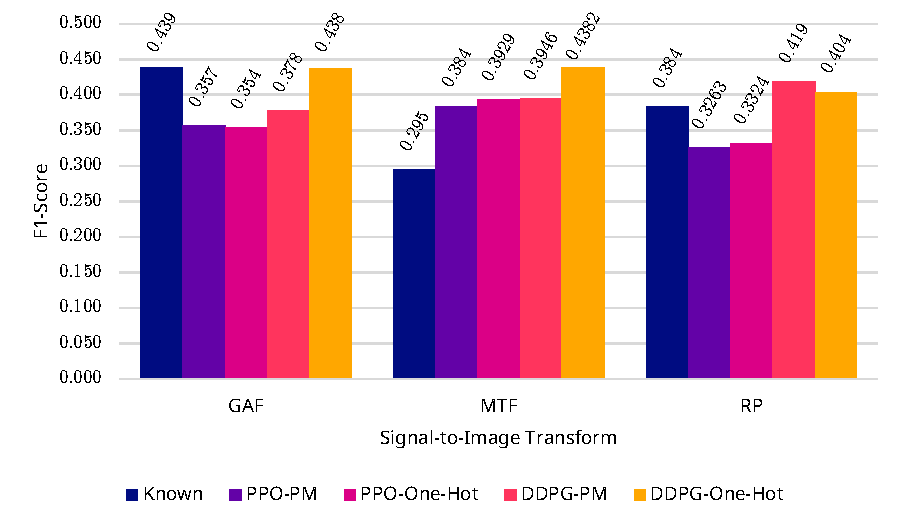
\includegraphics[width=6in]{figures/results_main}
	\caption{The summarized results of the experiments, showing F1-score grouped by the signal-to-image transform used. For each signal-to-image transform, the colors represent the RL algorithm and the encoding used.}
	\label{fig:results-main}
\end{figure}

\begin{figure}
	\centering
	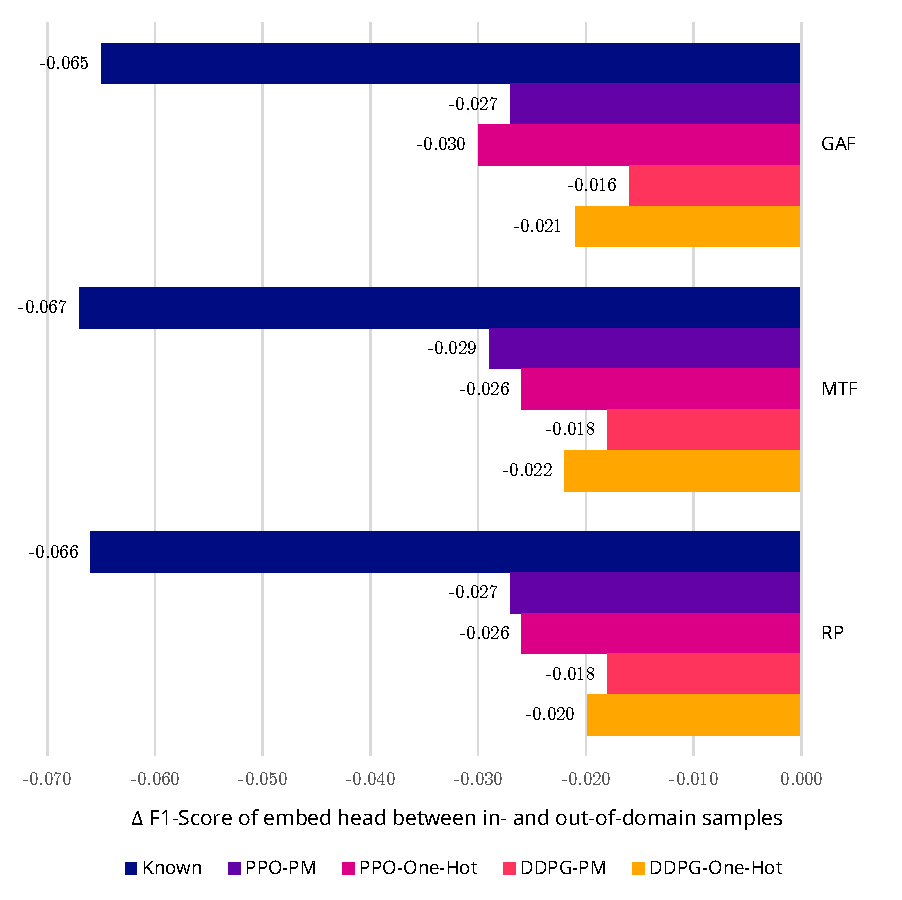
\includegraphics[width=6in]{figures/results_domains}
	\caption{The difference in performance of our models on in-domain vs. out-of-domain samples. The in-domain samples were taken from a held-out set of the training samples. The values are grouped by signal-to-image transform and the colors represent the RL algorithm and the encoding used. The shown values indicate the reduction in F1-score of our model on out-of-domain samples w.r.t. the in-domain samples with lower values indicating better performance on the in-domain samples.}
	\label{fig:results-domains}
\end{figure}
	
\begin{figure}
	\centering
	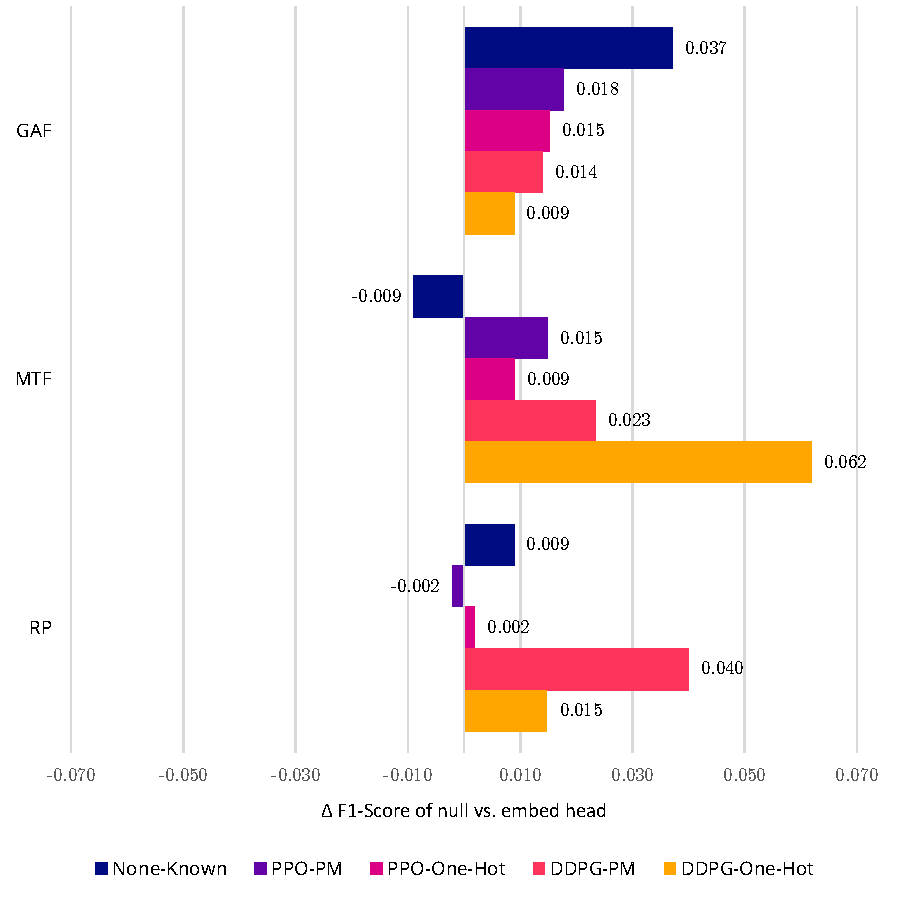
\includegraphics[width=6in]{figures/results_delta}
	\caption{This chart shows the performance delta between the null head and the embed head for each experiment. Higher positive values indicate that the embed head achieved a higher F1-score.}
	\label{fig:results-delta}
\end{figure}

\begin{figure}
	\centering
	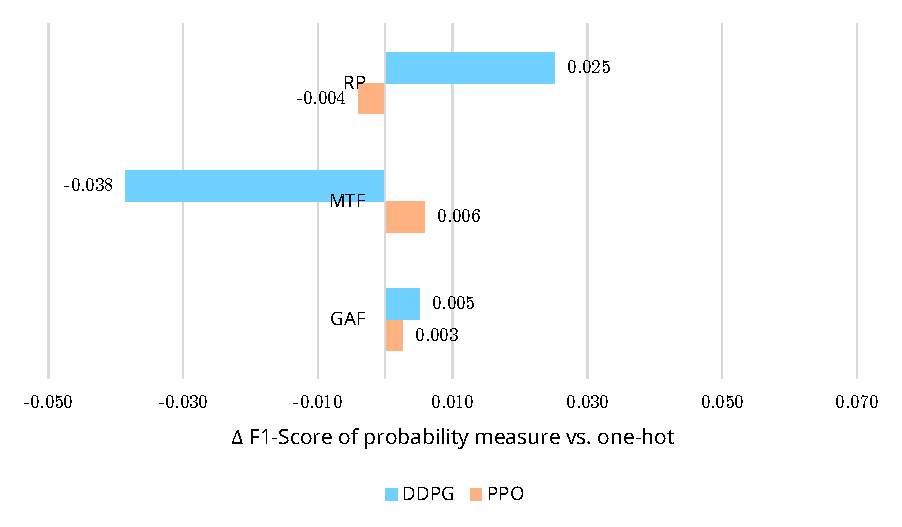
\includegraphics[width=6in]{figures/results_encoding}
	\caption{This chart shows the overall performance delta between using a probability measure and a one-hot encoding for the domain embedding. The values are grouped by signal-to-image transform and the colors represent the RL algorithm used. The scores used here have also been corrected for their respective algorithm's null head performance, i.e., uses the scores seen in Figure \ref{fig:results-delta} instead of in Table \ref{tab:final-results}. Higher positive values indicate the embed head achieved a higher F1-score when using the probability measure encoding as opposed to using a one-hot encoding.}
	\label{fig:results-encoding}
\end{figure}

To answer our research questions, we set up a series of experiments with single-user leave out validation.
The criteria used to choose which samples were used as training samples and which for testing are shown in Table \ref{tab:single-user-select} and resulted in a $\frac{2}{3}:\frac{1}{3}$ split of the data.
We additionally held $\frac{1}{10}$ of the training data as a hold-out split to test in- vs.\ out-of-domain performance of our model.
We chose these specific users due to them all being males of similar BMI, as seen in Figure 12 of \cite{zheng2019zero}.
Using this data, we set up experiments to answer our research questions from Section \ref{sec:intro-problem-statement}.
These experiments ran every combination of RL agent (PPO, DDPG, and known domain factors as a baseline), signal-to-image transform (GAF, MTF, and RP), and encoding method (probability-measure and one-hot) that we have previously chosen.

The results of our experimental runs can be seen in Table \ref{tab:final-results} and are visualized in Figure \ref{fig:results-main}.
This table, and every figure with experimental results, shows the final model performance on the test set.
In this table, we show the performance of DARLInG with two RL algorithms: PPO and DDPG, as well as when the embed head is provided the known domain factors.
For each embedding type, we encode the output as either a probability measure (PM) or as a one-hot encoded vector.
Finally, for each algorithm and encoding, we provide an input image of the CSI as transformed by GAF, MTF, and RP, details of which can be found in \ref{sec:background-signal-to-image}.

Another way to analyze our runs is to investigate the difference in performance of our model on in-domain vs. out-of-domain samples.
To do so, we ran our trained models on the held-out split of the training set.
The results can be seen in Figure \ref{fig:results-domains}.
These results indicate that in all cases, our model performs better on in-domain samples, as is expected.
The performance on out-of-domain samples are much worse on the known encoding, indicating that the known encoding of domain factors, while usable, is not great for out-of-domain samples.
Our results also support that DDPG performs best for out-of-domain samples.

The performance of the embed heads compared to their respective null heads can be seen in Figure \ref{fig:results-delta}, in which greater positive values indicate that the embed head is performing better than the null head.
We can see that with MTF and RP, DDPG out-performs PPO while PPO slightly outperforms DDPG with GAF.
Using known domain factors improves performance, but only with GAF and RP transforms while it has the decreases performance with MTF.
The largest increase in performance can be seen with MTF transforms and the DDPG RL algorithm with one-hot encoding.
Interestingly, PPO with RP seems to provide no actual benefit.

To answer our second research question, we compare the performance of a domain embedding encoded as a probability-measure and one using one-hot encoding, the results of which are seen in Figure \ref{fig:results-encoding}.
The results show that generally, the encoding method does not make a significant difference for PPO and only makes a difference for DDPG with MTF and RP transforms.
With the MTF transform, one-hot is the preferred encoding while in RP, the probability-measure is the prefered encoding.

Comparing all these results with the baseline of a known domain encoding, we see that although the known-domain encoding performs well with GAF and RP, and poorly on MTF, the known-domain encoding fails to provide an adequate representation of out-of-domain samples, as seen in Figure \ref{fig:results-domains}.
This may simply be to the discrete (i.e., categorical) encoding of the domain factors provided by the known domain encoding, instead of the more complex domain representations provided by the RL agents.
For example, although subject height is a continuous variable which can be properly encoded by a multi-dimensional one-hot encoding or a probability measure, a one-hot user encoding provides no further information about how height varies between two users.
This suggests that the RL agents provide a better encoding across domains, but fall short of hand-crafted domain labels with ground-truth information and no out-of-domain samples.

The results are generally unimpressive, though, with F1-scores significantly below both the baseline in \cite{zheng2019zero} and any of the state-of-the-art methods discussed in Chapter \ref{chapter:literature-review}.

\subsection{Extended Run}\label{subsec:experiments-longer}

\begin{table}[]
	\centering
	\begin{tabular}{@{}lr@{}}
		\toprule
		         & F1-Score \\ \midrule
		Standard & 0.438    \\
		Extended & 0.553    \\ \bottomrule
	\end{tabular}
	\caption{Extended training run results of the DDPG agent with MTF transform and one-hot encoding.}
\end{table}

As one final experiment, we ran our best performing configuration, i.e., DDPG with MTF transform and one-hot encoding, on the TU/e High-Performance Computing cluster with 100 model epochs and 50400 agent iterations per epoch.
The number of agent iterations were chosen as the closest full dataset iterations to 50000 steps, resulting in a total of 3528000 total agent steps as we set the agent training starting epoch $\zeta = 30$.
We double $\zeta$ to 30 as we also double the total number of epochs during training.
This is twice the training length of the VAE and 100$\times$ the training length for the agent relative to the other training runs.

We observe an increase in performance, with an increase in F1-score of 0.12 and the performance plateauing around epoch 75.
Although this is a welcome increase in performance, this is still below the baselines in \cite{zheng2019zero} and any of those discussed in Chapter \ref{chapter:literature-review}.
The performance plateauing after epoch 75 does suggest that increasing training duration any further will most likely not increase model performance.

\chapter{Discussion}

We have shown that our approach is capable of generally improving F1-scores in Widar, but our overall performance is disappointing, compared to both baselines and state-of-the-art approaches.
In this chapter, we discuss the experimental results and what these results mean with respect to our research questions, analyze the latent space and domain embeddings produced by our approach, as well as suggest future research that may be taken.

\section{Comparison to State-of-the-Art}

\begin{figure}
	\centering
	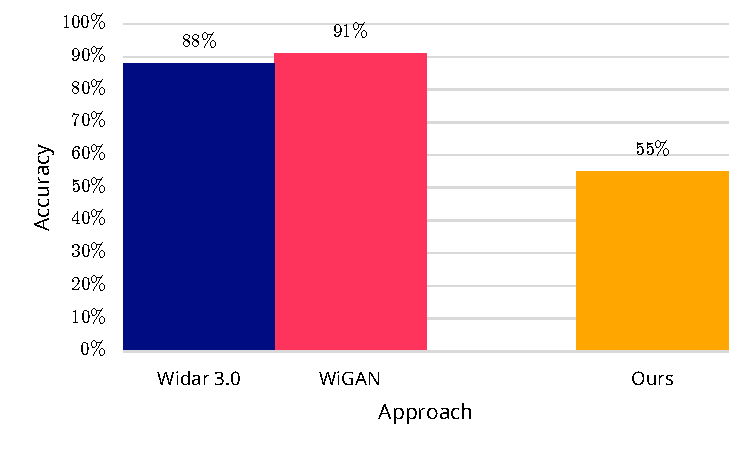
\includegraphics[width=5in]{figures/results_sota}
	\caption{Comparison of our method against the Widar 3.0 benchmark and the current SOTA. The space between our work and other works is intentionally placed to reiterate the point that these values are not directly comparable as our data splits, although both representing single-user leave-out, are not comparable.}
	\label{fig:results-sota}
\end{figure}

It is difficult to compare our results to the state-of-the-art (SOTA), as we did not train on the same training splits as those SOTA models.
We can, though, make a rough comparison to the CNN baseline in the Widar 3.0 paper \cite{zheng2019zero} and to the WiGAN approach in \cite{jiang2020wigan}.
Both these papers provide results for single-user leave-out and the performance comparison with our method can be seen in Figure \ref{fig:results-sota}.
In the Widar 3.0 paper, the CNN approach used is able to provide a baseline result of $88\%$ accuracy in single-user leave-out while 
WiGAN is able to achieve $91\%$ accuracy.
These methods both provide significantly better results than DARLInG, which achieves a best performance of $55\%$ accuracy when using DDPG with MTF.

It should be reiterated, though, that these numbers are not directly comparable as they do not use the same dataset splits.

\section{Research questions}

In this section, we answer each of the research questions we posited in Section \ref{sec:intro-problem-statement} as well as a short discussion on the strengths and limitations of our approach to answering these questions.

\paragraph{Research Question 1}
Our first question asks how well DARLInG's embed heads perform compared to its null heads.
The results from Table \ref{tab:final-results} indicate that we were able to achieve up to 7.1 percentage points of improvement on accuracy and an improvement on the F1-score of 0.062 when comparing the null head and the embed head on out-of-domain results.
This was found when using MTF as the transform, DDPG as the RL agent, and one-hot encoding as the domain embedding encoding.
The results when run with other configurations indicate that the magnitude of the performance increase may not be as large, although it is generally positive.

The only configuration where there was a performance decrease was with PPO using the RP transform.
With this configuration, the $\Delta$ F1-score was -0.002 for the PM encoding and +0.002 for the one-hot encoding.
As such, we conclude that this was a negligible difference and should therefore be interpreted as DARLInG not having any effect on model performance.

We therefore conclude that our results suggest using DARLInG to provide unsupervised domain labels provide similar or better out-of-domain performance on Widar.

\paragraph{Research Question 2}
Our second question asks how changing the domain embedding encoding affects performance.
Generally, DDPG seems to perform better when using a PM encoding when the transform is RP while it performs better with one-hot encoding when the transform is MTF.
For all other combinations, the results in Figure \ref{fig:results-encoding} show no significance difference in performance between encodings.
As a result, we believe that the domain embedding is not significant and that other factors contribute more towards the performance of the model.
Further research may be necessary to investigate the optimal encoding of the domain embedding.

\paragraph{Research Question 3}
Our last research question asks how changing the signal-to-image transformation affects performance.
Our results indicate that generally, GAF performs consistently, but not impressively.
MTF seems to perform quite well with DDPG and similarly to GAF with PPO.
RP seems to perform poorly with PPO, not improving over the null head, while performing similarly to MTF with DDPG.
As a result, we can confidently conclude that different signal-to-image transformations affect model performance, but the results are inconclusive as to which transformation works best.
The results do suggest, though, that MTF may be the best performer in our experiments of limited sample size.

\paragraph{Strengths and Limitations}
We believe that our experiments are quite thorough with significant resources put into ensuring that the model itself is working appropriately, as well as that the code is free of any significant bugs which could render the results invalid.
Significant effort was put into ensuring that every step of the CSI processing and transformation pipeline produced the correct results during the course of writing the thesis.
The VAE was also checked by running the VAE with the Fashion-MNIST dataset \cite{xiao2017fashion}.
This produced results as expected with the VAE being able to adequately reconstruct the input images as well as classify the images appropriately with $>0.85$ accuracy, matching the benchmarks in \cite{xiao2017fashion}.
Finally, the RL algorithms used are off-the-shelf implementations from Stable Baselines 3 \cite{raffin2021stable} implemented according to the sample code provided, reducing the likelihood of issues in the code with the RL algorithms.
We also approached a PhD candidate at the TU/e specializing in RL who concurred with our ideas on the alternating training style, where we iterate between training the RL agent and the VAE \cite{grooten2023interview}.

Limitations include reduced hyperparameter tuning of the RL agents.
RL agents are notoriously time-consuming to train \cite{schulman2017proximal,schulman2017trust,lillicrap2015continuous}.
With our limited compute resources, we were unable to conduct a full hyperparameter optimization sweep of the RL agents.
We used known good hyperparameters provided in the documentation of \cite{raffin2021stable} for dealing with a continuous action space for our agents.

\section{Latent Space and Domain Embedding Analysis}\label{sec:discussion-ls-de-analysis}

\begin{figure}
	\centering
	\begin{subfigure}{0.3\textwidth}
		\centering
		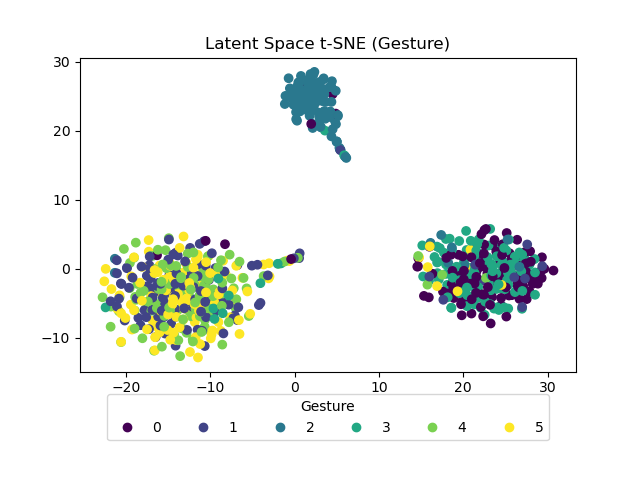
\includegraphics[width=\textwidth]{figures/mtf-ppo-one/ls-gesture}
		\caption{t-SNE by gesture}
		\label{fig:mtf-ppo-one-ls-gesture}
	\end{subfigure}
	\hfill
	\begin{subfigure}{0.3\textwidth}
		\centering
		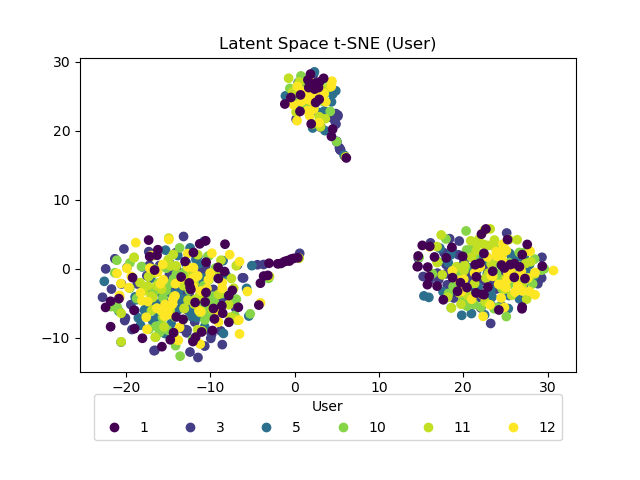
\includegraphics[width=\textwidth]{figures/mtf-ppo-one/ls-user}
		\caption{t-SNE by user}
		\label{fig:mtf-ppo-one-ls-user}
	\end{subfigure}
	\hfill
	\begin{subfigure}{0.3\textwidth}
		\centering
		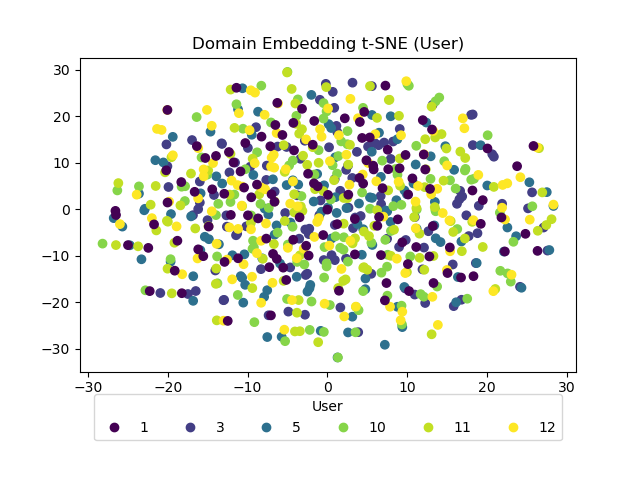
\includegraphics[width=\textwidth]{figures/mtf-ppo-one/de-user}
		\caption{t-SNE by User}
		\label{fig:mtf-ppo-one-de-user}
	\end{subfigure}
	\caption{t-SNEs of the latent space and domain embeddings produced by PPO with one-hot encoding and MTF transformation.}
	\label{fig:mtf-ppo-one}
\end{figure}
\begin{figure}
	\centering
	\begin{subfigure}{0.3\textwidth}
		\centering
		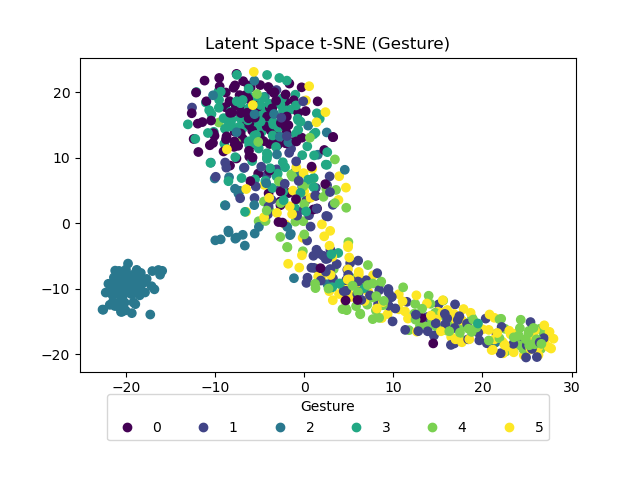
\includegraphics[width=\textwidth]{figures/mtf-ppo-pm/ls-gesture}
		\caption{t-SNE by gesture}
		\label{fig:mtf-ppo-pm-ls-gesture}
	\end{subfigure}
	\hfill
	\begin{subfigure}{0.3\textwidth}
		\centering
		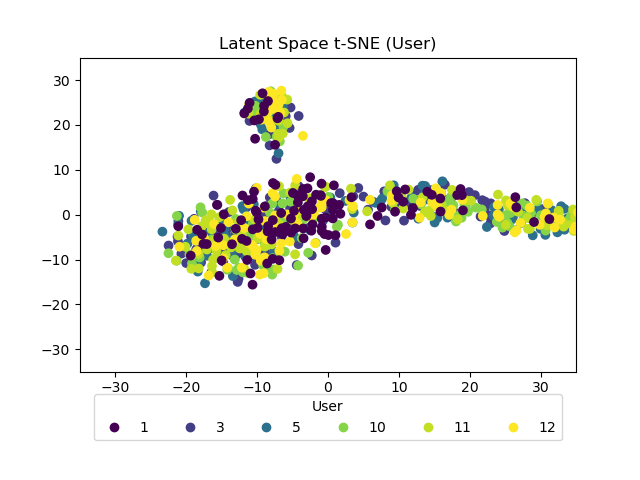
\includegraphics[width=\textwidth]{figures/mtf-ppo-pm/ls-user}
		\caption{t-SNE by user}
		\label{fig:mtf-ppo-pm-ls-user}
	\end{subfigure}
	\hfill
	\begin{subfigure}{0.3\textwidth}
		\centering
		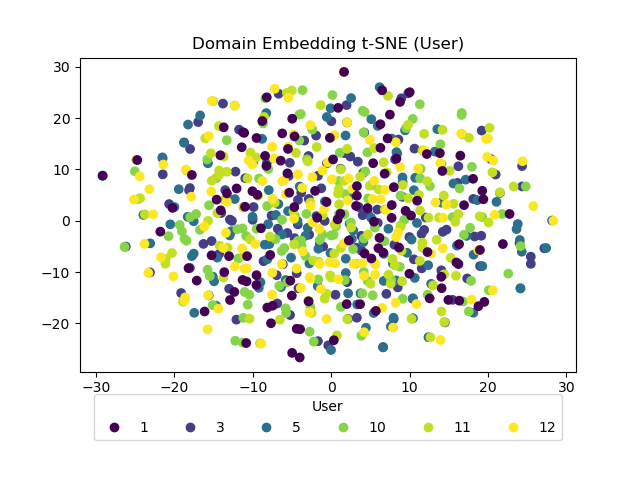
\includegraphics[width=\textwidth]{figures/mtf-ppo-pm/de-user}
		\caption{t-SNE by user}
		\label{fig:mtf-ppo-pm-de-user}
	\end{subfigure}
	\caption{t-SNEs of the latent space and domain embeddings produced by PPO with PM encoding and MTF transformation.}
	\label{fig:mtf-ppo-pm}
\end{figure}

To properly analyze the low performance of our model, we would like to analyze both the latent space $\boldsymbol{z}$ produced by our encoder as well as the domain embeddings $\boldsymbol{d}_{r}$ produced by our RL agent.
We do this by running the entire dataset through both the encoder and RL agent and produce t-SNE embedding plots with their outputs.
By doing so, we can see if there is any structure to the embeddings.
We specifically analyze the case of using MTF as the signal-to-image transformation, PPO as the agent, and both the one-hot and probability measure domain embedding encodings, the results of which can be seen in Figures \ref{fig:mtf-ppo-one} and \ref{fig:mtf-ppo-pm}.

We can see that for the latent space, there is a much clearer structure in both configurations, especially with gesture 2 being separated out quite distinctly in both Figures \ref{fig:mtf-ppo-one-ls-gesture} and \ref{fig:mtf-ppo-pm-ls-gesture}. 
Interestingly, both Figures \ref{fig:mtf-ppo-one-de-user} and \ref{fig:mtf-ppo-pm-de-user} show quite an even distribution of users throughout each cluster in the t-SNE space.

For the domain embeddings, we see that there is \textit{some} structure in Figures \ref{fig:mtf-ppo-one-de-user} and \ref{fig:mtf-ppo-pm-de-user}, as it is not only a single normally-distributed disk, but there is not much of it.
We also see that the users, including the single-leave out user (User 1) is distributed quite evenly throughout the space in both figures.
This suggests that the RL agent is not able to accurately provide significantly different domain embeddings between the users.
We believe this may be simply due to training time constraints.

\begin{figure}
	\centering
	\begin{subfigure}{0.3\textwidth}
		\centering
		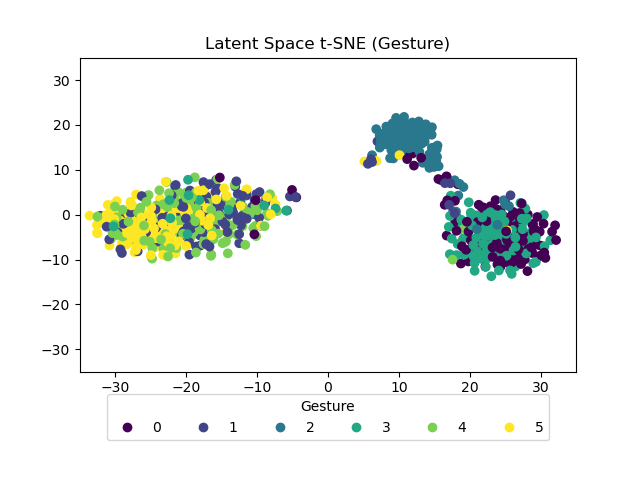
\includegraphics[width=\textwidth]{figures/extended/long_ls_gesture}
		\caption{t-SNE by gesture}
		\label{fig:extended-ls-gesture}
	\end{subfigure}
	\hfill
	\begin{subfigure}{0.3\textwidth}
		\centering
		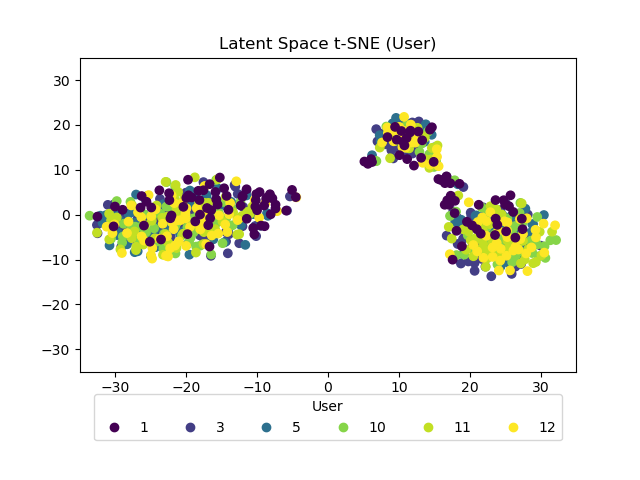
\includegraphics[width=\textwidth]{figures/extended/long_ls_user}
		\caption{t-SNE by user}
		\label{fig:extended-ls-user}
	\end{subfigure}
	\hfill
	\begin{subfigure}{0.3\textwidth}
		\centering
		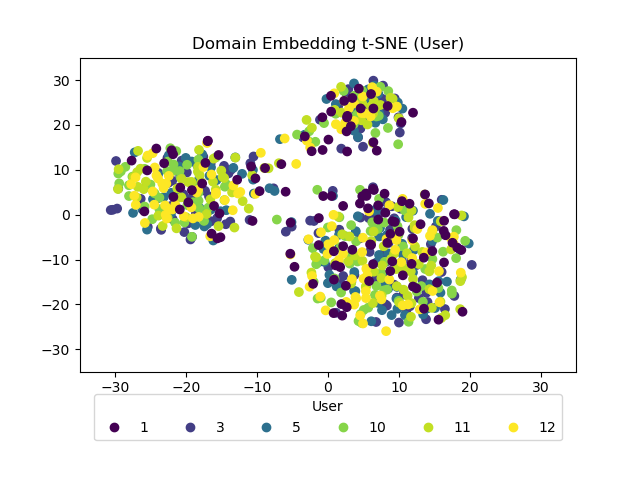
\includegraphics[width=\textwidth]{figures/extended/long_de_user}
		\caption{t-SNE by user}
		\label{fig:extended-de-user}
	\end{subfigure}
	\hfill
	\begin{subfigure}{0.3\textwidth}
		\centering
		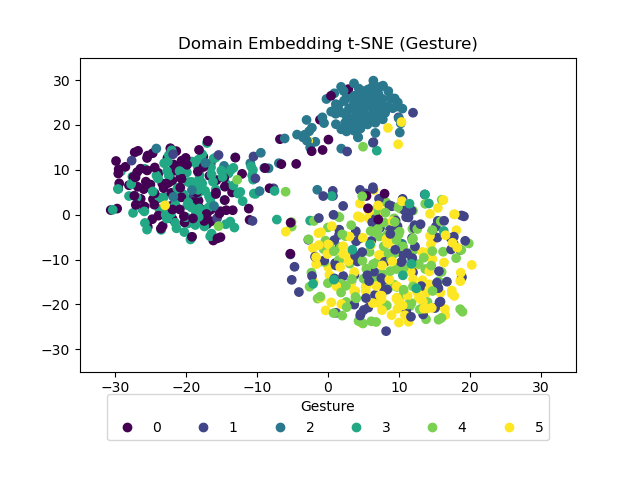
\includegraphics[width=\textwidth]{figures/extended/long_de_gesture}
		\caption{t-SNE by gesture}
		\label{fig:extended-de-gesture}
	\end{subfigure}
	\hfill
	\caption{t-SNEs of the latent space and domain embeddings produced by PPO with one-hot encoding and MTF transformation with extended training time.}
	\label{fig:extended-tsnes}
\end{figure}

To test this hypothesis, we trained our agent for an extended period of time, as was described in Subsection \ref{subsec:experiments-longer}.
The t-SNEs of this run can be seen in Figure \ref{fig:extended-tsnes}.

We notice some clearer separation by gesture in Figure \ref{fig:extended-ls-gesture}, with gestures 2 and 0 being more clearly separated on the right side clusters.
Additionally, Figure \ref{fig:extended-ls-user} shows some more clustering within clusters for the users. For example, user 1 is primarily clustered towards to the top of the left-side cluster, for example.
Finally, we finally see some structure brought to the domain embeddings, with 3 clearly visible clusters in Figure \ref{fig:extended-de-user}, although they do not seem to correspond to the users themselves.

We additionally plotted the domain embedding t-SNE colored by gesture in Figure \ref{fig:extended-de-gesture}, and we notice that the domain embeddings are instead clustered by gesture.
This is interesting, as it means that our domain embeddings are in fact directly providing data on the gesture for the embed head, instead of simply providing data about the domain.
This would imply that we have some sort of meta-model made up of the embed head and the RL agent which together attempt to provide better gesture classifications.

We also plotted the domain-embedding t-SNE colored by gesture for both short run configurations, but we see no such clustering in those and as such, for brevity, will not include the plots.

We also plotted the latent-space and domain embedding t-SNEs, filtered by user and colored by gesture to analyze whether this provides any additional insight.
After analyzing these plots, we do not see any additional insight that can be taken from them, but nonetheless they are available in Appendix \ref{appendix:tsne}.

\section{Future Research}

We believe that there may still be potential in our approach.
Further research could be aimed at a different neural-network architecture, tuning of the RL agents and some changes to the training regime.

\subsection{A Different Architecture}

Although our preliminary experiments in Section \ref{sec:experiments-preliminary} suggested that our VAE model could perform adequately for the task of gesture classification with Widar, it was evidently not up to the task of gesture classification where the input is domain shifted.
One may, instead of using a VAE, use one of the known performant models from Section \ref{sec:literature-csi-for-gesture}.
This may result in better cross-domain performance to begin with with our RL approach adding the few percentage-points on top to make said models competitive with single-domain models.

\subsection{Tuning of the RL Agent}

Due to time constraints, we conducted little hyperparameter tuning of the RL agent due to time and compute constraints. 
Future research may simply repeat our experiments but with increased time and compute to see if that could help at all.

We might also develop a different reward function which forces the agent to provide a domain embedding which more clearly provides additional information about the domain itself, instead of additional information about the gesture as our agent seems to have done as seen in the analysis in Section \ref{sec:discussion-ls-de-analysis}.

\subsection{A Different Training Regime}

Finally, we see in the loss curves of our experiments that there is a always a sudden increase in the loss function of the model, with a corresponding drop of around 0.05—0.10 in validation accuracy of the null head, at the epoch in which we introduce the embed head.
This decrease in validation accuracy of the null head may indicate that the changes our model makes to the latent space while trying to optimize for the embed head and RL agent is adversely affecting the performance of the null head.
Put another way, the null head is not capable of adapting to the changes in the latent space which the model makes while trying to optimize for the embed head.
We suggest that future work could look into two different approaches to this problem: By training the embed head as a completely separate model on a frozen encoder, or by changing the way we train the embed head using a process we propose called Simulated Aging and Hardening.

It might be possible to reduce the decrease in performance of the null head, and potentially increase overall performance, by training the embed head as an entirely separate network to the encoder and null heads.
In this approach, during the VAE training portion of every epoch, the encoder and null head would first be trained over the entire training set.
After every batch has been processed and the optimizers run for the encoder and null head, the parameters of said modules would be frozen.
At this point, we will start optimization on the embed head.
The same training set will be run through the encoder again and the produced outputs $\boldsymbol{z}$ along with the produced domain embeddings $\boldsymbol{d}_r$ from the RL agent (also frozen) would be run through the embed head to produce its gesture class predictions.
This would ensure that the embed head is being trained to predict only based on the $\boldsymbol{z}$ and $\boldsymbol{d}_r$ without affecting the encoder or the null head.
Then finally, with everything frozen, we train only the RL agent.
By doing so, the RL agent is forced to learn from an environment which is not itself adapting to the actions of the agent, potentially simplifying the environment evolution for the agent.

We might also attempt to instead slowly increase the rate of optimization of the embed head in a process we propose to be called \textit{Simulated Aging and Hardening} (SAH), directly inspired by the analogy used by simulated annealing (SA) to metallurgy.
In SA, we use an initial solution and probabilistically explore neighboring solutions with exploratory probability. 
Over time, we slowly ``cool down'' the probability of accepting worse solutions until we arrive at a near-optimal solution.
In this way, SA can be said to start of very exploratory and slowly reduce its exploration and increase its exploitation of known good solutions.
Conversely, our proposed SAH follows the process of aging and hardening, a process in metallurgy with similar results to annealing but with opposite processes.
The steps to hardening in metallurgy is typically as follows: Start with a metal that is at a high temperature, quench it to rapidly cool it down ``freezing'' the alloying elements in the metal, and finally slowly heat up the metal in a process called aging and hardening.

In SAH, applied directly to our use case, we would train the encoder and null heads in the same way we do now until the epoch where the embed head and RL agent starts training.
At this point, we would freeze the training of the encoder and null heads.
The embed head is then initialized with a copy of the parameters of the null head.
As the parameters are equivalent, it is unlikely to be able to process input from the RL agent properly.
We start off by using a low learning rate on the embed head to avoid sudden large changes to its parameters and avoiding instability while looking for the new minima.
After a certain number of epochs, or some heuristic is reached, we then continue training the model as a whole with the current training method described in this thesis.

\chapter{Conclusions}\label{chapter:conclusions}

Write your conclusions here.

\printbibliography

\appendix
\addcontentsline{toc}{chapter}{Appendix}

%\chapter{Appendices}
%In this file (appendices/main.tex) you can add appendix chapters, just as you did in the thesis.tex file for the `normal' chapters.
%You can also choose to include everything in this single file, whatever you prefer.

\chapter{Plan}

The plan involves of the following steps, which are elaborated upon in the Gantt Chart seen in Table \ref{fig:plan-gantt-chart}.

\begin{enumerate}
	\item Initial infrastructure setup. This involves building the train-validate-test loops, building the data ingest/transformation pipelines, and building the model-building pipelines. This is feasible in the given timespan since much of the code will be taken from the IRIS Seminar project.
	\item Integration of all modules as well as integration of hyperparameter optimization and training-tracking code complete. Initial training/debugging of the network can begin.
	\item Parallelization of reinforcement-learning and deep-learning components of the network are complete. This involves making it possible to run the RL and the DL models on separate computers during training, if this improves performance.
	\item Get initial results, bugs will be found and ``beta-testing'' of the framework starts. All results at this point are taken with a massive grain of salt since something will cause the results to be wrong, speaking from experience.
	\item Deeper investigations through hyperparameter optimization and changes to the model architecture should now start or is already ongoing.
	\item Final results from the experiments should be completed.
	\item First draft of the paper.
	\item Second draft the paper.
	\item Final draft of the paper.
	\item Thesis defense preparation.
\end{enumerate}

\begin{figure}
	\centering
	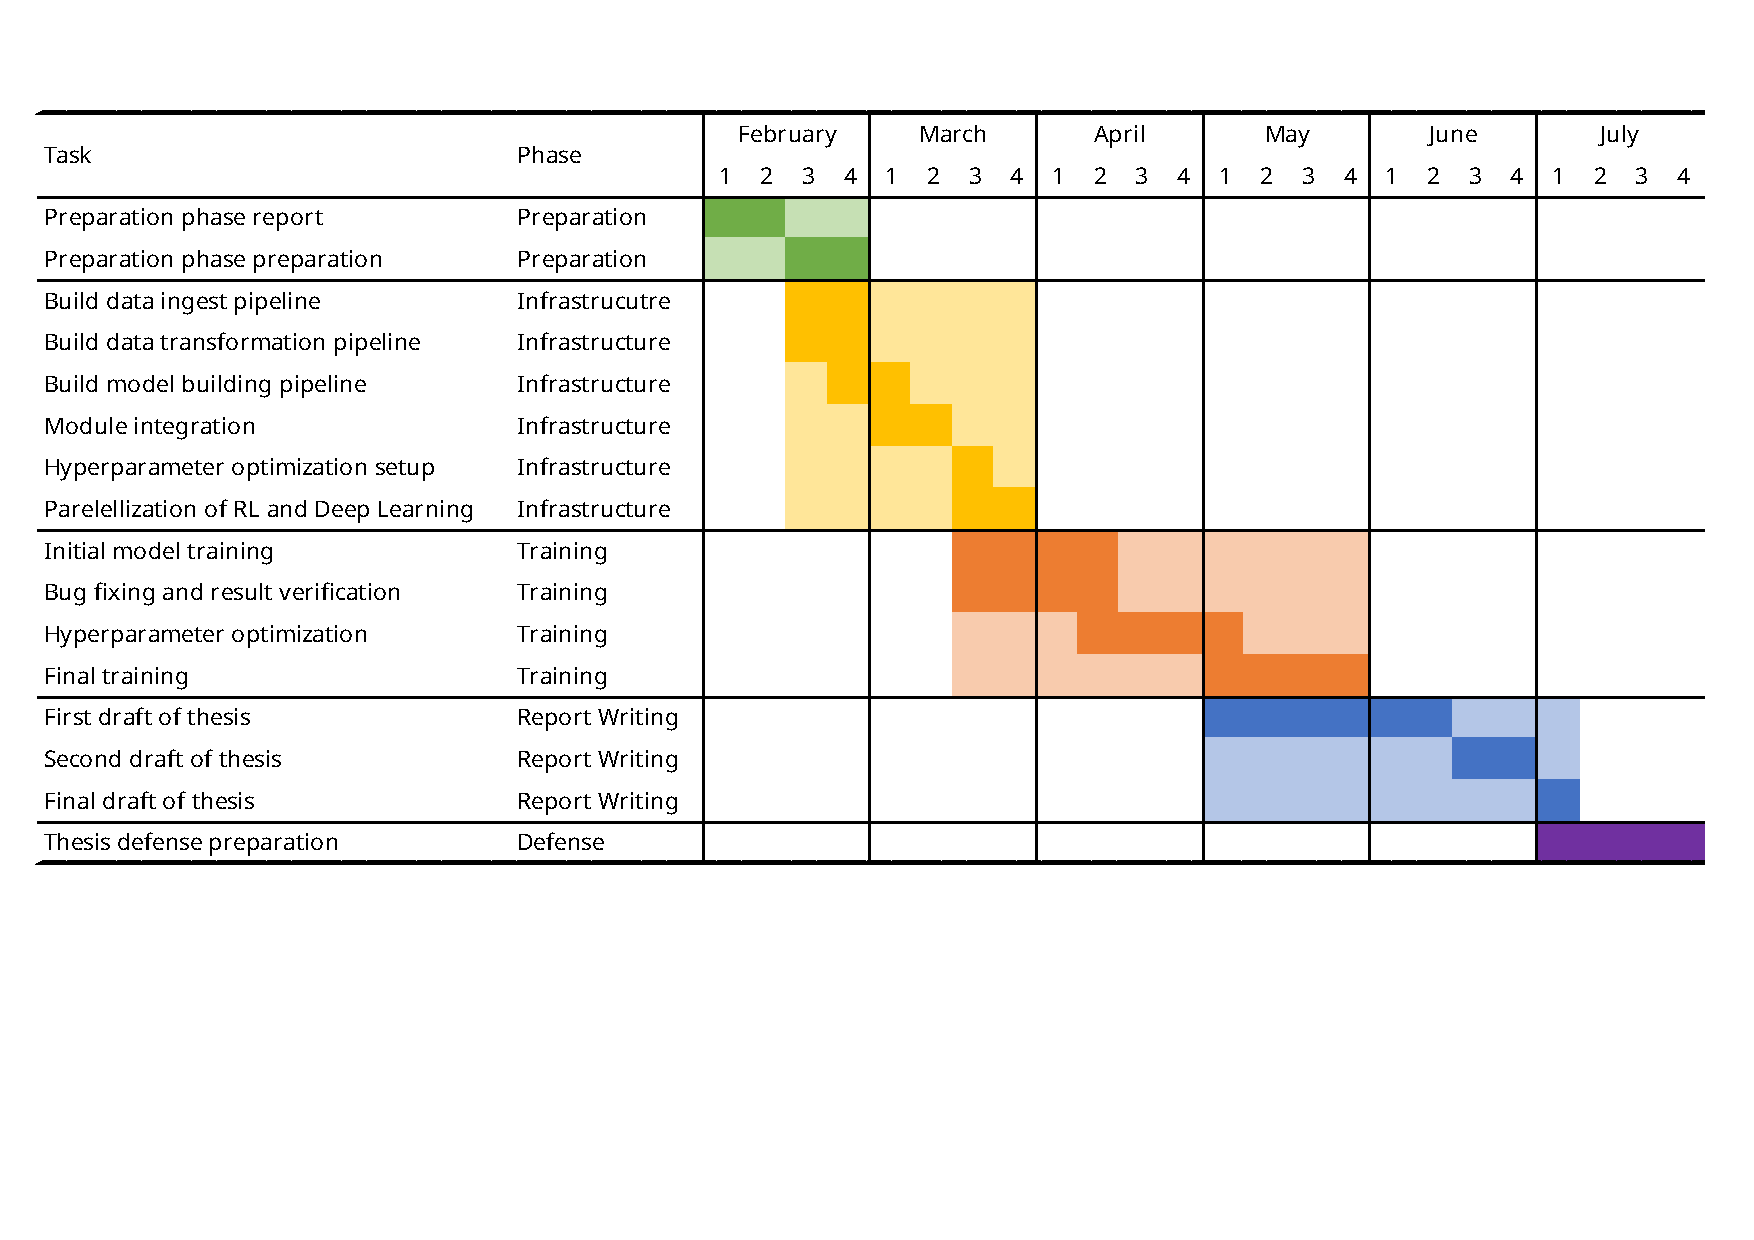
\includegraphics[width=\textwidth,trim={0.5cm 5cm 0.5cm 1cm},clip]{figures/gantt_chart}
	\caption{A Gantt chart showing the plan for this thesis}\label{fig:plan-gantt-chart}
\end{figure}
\chapter{Risk Assessment}

Risks identified for each phase of the plan and mitigation options are investigated in this section.
Risk mitigation strategies are built from the author's previous experience working in an AI research lab and as a data scientist and software developer in industry.
Additionally, strategies are also developed from theory learned in his computer science bachelor's.

\paragraph{Initial infrastructure setup}
During the initial infrastructure setup, the entire pipeline will be developed.
This includes a modular data-ingest/transformation pipeline and model-building pipeline.
Risks include data availability/usability and bugs in the data pipeline code.
Additionally, the model will be completely modular and not prebuilt, increasing the chances of a bug appearing during this building phase but increasing flexibility of the model being investigated.

Data availability/usability refers to the fact that while the data is a public and published dataset, it is nonetheless quite large and it would not be feasible to download the entire dataset and place it on TU/e's HPC server. 
This means that some way to compress the data must be done.
It is also possible that the transformed version of the data can be compressed more efficiently and this is what will end up being the dataset we work with for the majority of the project.

The data pipeline is also modular, allowing for data augmentation to be added ``on-the-fly'' instead of being hard-coded.
This increases flexibility, but introduces the risk of bugs in unexpected circumstances.
Mitigation factors include having written similar pipelines multiple times in the past and reuse of old, known-good code from the IRIS Seminar project and 2AMM10 Deep Learning course.
Additionally, a similar approach has been use in previous research that we have completed, and we have significant experience in similarly modular pipelines.

Similarly, the model is built only at run-time, allowing for more flexibility and the possibility to fine-tune the model architecture using hyperparameter optimization techniques.
This increases the chance that a good model architecture is chosen and strengthens the reasoning behind the chosen model architecture through empirical performance.
Mitigation factors are the same as for the data pipeline.

\paragraph{Module Integration}
The most complex part of this infrastructure is to ensure that all modules work well together and there are no bugs in the hand-off step between modules.

To mitigate these factors, we take some advice from Chip Huyen's book Designing Machine Learning Systems \cite{dmlsbook2022}.
To ensure that errors are not made during this integration, data flow will be closely monitored and visualized at every step through a UI, such that it is easy to see if anything went wrong at any step.
The application of this will essentially be most of the interim steps being given some sort of output so we can visualize their result and track how data is transformed throughout the entire process.

\paragraph{Parallelization}
This is potentially unnecessary and may take up time that could be better used elsewhere.
The idea is essentially that it might make sense to have the reinforcement-learning model and the gesture-classification model run on separate computers and having them communicate through some network.

Mitigation for this being unnecessary is providing only a limited amount of time to do this and the understanding that if this seems too difficult/may take too long, then we will immediately shelf the idea.

\paragraph{General bugs}
As with any software-based project there will inevitably be bugs in the code.
Software engineering principle which lead to fewer bugs, such as proper use of debugging tools (but not test suites as we don't believe they will be necessary for a project with a limited scope such as this), will be used throughout work on this thesis.
Additionally, use of ``magic numbers'' will be limited and as many parameters as appropriate will be assigned from variables.


\end{document}
